\documentclass[review]{elsarticle}

\usepackage{lineno,hyperref}
\usepackage{bm}
\usepackage{float}
\usepackage{subfig}
\usepackage{color}
\usepackage{amsmath}
\usepackage{amssymb}
\usepackage{multirow}
\usepackage{graphicx}
\usepackage{rotating}
\usepackage{array}
\usepackage[export]{adjustbox}
\usepackage{lineno,hyperref}
\usepackage[T1]{fontenc}
\usepackage[utf8]{inputenc}
\usepackage[table]{xcolor}
\usepackage{caption}
%\usepackage{subcaption}
\usepackage{graphicx}
\modulolinenumbers[5]
\usepackage[margin=1.5in]{geometry}
%\journal{Journal of \LaTeX\ Templates}

%% `Elsevier LaTeX' style
\bibliographystyle{elsarticle-num}


\begin{document}
%		\fontfamily{qtm}\selectfont
\begin{frontmatter}

\title{Accelerated Magnetic Resonance Imaging by Generative Adversarial Neural Networks}

%% Group authors per affiliation:
\author{Ohad Shitrit, Tammy Riklin Raviv}
\address{$^1$Department of Electrical Engineering, 
	     $^2$The Zlotowski Center for Neuroscience
	     Ben-Gurion University of the Negev, Israel}


\begin{abstract}
A main challenge in Magnetic Resonance Imaging (MRI) is speeding-up scan time. Beyond the improvement of patient experience and the reduction of operational costs, faster scans are essential for time-sensitive imaging, such as fetal, cardio or functional MRI, where temporal resolution is important and target movement is unavoidable, yet must be reduced. Current MRI acquisition methods speed-up scan time at the price of lower spatial resolution and costly hardware.
We introduce a practical, software-only framework, based on deep learning, for accelerating MRI acquisition, while maintaining anatomically meaningful imaging. This is accomplished by MRI sub-sampling, while using a generative adversarial networks to directly estimate the missing k-space samples. The generator-discriminator inter-play enables the introduction of an adversarial cost in addition to fidelity loss used for optimizing the reconstruction. Promising results are obtained for up to six-fold acceleration of diverse brain MRIs, from a large publicly available dataset. Clinical usability of the reconstructed images is assessed by performing tissue segmentation and comparing the results to those obtained by using the original fully-sampled images. Segmentation compatibility, measured in terms of Dice scores and Hausdorff distances, demonstrate the quality of the proposed MRI reconstruction with respect to other methods, including the widely-used compressed sensing.
\end{abstract}

\begin{keyword}
	\text Accelerated MRI \sep Adversarial Loss \sep Deep Neural Network \sep K-space
	%\MSC[2010] 00-01\sep  99-00
\end{keyword}

\end{frontmatter}

\linenumbers


\section{Introduction}
Magnetic Resonance Imaging (MRI) is a non-ionizing imaging modality, and is therefore widely used in diagnostic medicine and biomedical research. The physical principles of MRI are based on a strong magnetic field and pulses of radio frequency (RF) electromagnetic radiation. 
Images are produced when hydrogen atoms, which are prevalent in living organisms, emit the absorbed RF energy that is then received by antennas in close proximity to the anatomy being examined. Spatial localization of the detected MRI signals is obtained by varying the magnetic field gradients. The discretized RF output is presented in a Fourier space
(called k-space), where the x-axis refers to the frequency and the y-axis to the phase. An inverse fast Fourier transform (IFFT) of the k-space is then applied for generating anatomically meaningful MRI scans. Figure \ref{fig:pair_of_k_space_mri} presents k-space traversal patterns used in conventional imaging. Each row of the k-space is acquired after one RF excitation pulse. The number of rows multiplied by the number of slices (z-axis) determines the total scan time.

The duration of standard single structural MRI acquisition is approximately 5 minutes. Usually, several scans of different modalities or a sequence of scans are acquired such that the overall scan time is much longer. The lengthy imaging process reduces patient comfort and is more vulnerable to motion artifacts. In cases where motion is inevitable, e.g., fetal MRI, cardiac cine, and lungs imaging, scan time must be significantly shortened, otherwise the produced images might be useless. Moreover, in dynamic MRI sequences, acquisition must be brief such that the temporal resolution of the sequence would allow capturing significant temporal changes, e.g., instantaneous increment of the contrast-enhanced material concentration in DCE-MRI or differences in hemodynamic response expressed in fMRI \cite{moeller2010multiband}.

A straight forward reduction of the scan time can be obtained by sampling fewer slices, thus reducing the spatial resolution in the z-axis. Spatial distances between adjacent slices of fetal MRI or fMRI, for example, are often as large as 0.5 centimeters. Therefore, a significant portion of the potential input is not acquired through imaging. On the other hand, under-sampling in the x-y domain leads to aliasing, as predicted by the Nyquist sampling theorem.

Numerous research groups as well as leading MRI scanner manufacturers make significant efforts to accelerate the MRI acquisition process. Hardware solutions allow parallel imaging by using multiple coils \cite{roemer1990nmr} to sample k-space data. There exist two major approaches~\cite{Deshmane2012} that are currently implemented in commercial MRI machines. Both reconstruct an image from the under-sampled k-space data provided by each of the coils. The sensitivity encoder (SENSE) transforms the partial k-spaces into images, then merges the resulting aliased images into one coherent image~\cite{pruessmann1999sense}. 
The GeneRalized Autocalibrating Partial Parallel Acquisition (GRAPPA) techniques~\cite{griswold2002generalized} operate on signal data within the complex frequency domain before the IFFT.

The compressed sensing (CS) technique~\cite{donoho2006compressed} allows efficient acquisition and reconstruction of a signal with fewer samples than the Nyquist-Shannon sampling theorem limit, when the signal has sparse representation in a known transform domain. Using CS for MRI reconstruction by sampling a small subset of the k-space grid had been proposed in~\cite{lustig2007sparse}. The underlying assumption is that the undersampling is random, such that the zero-filled Fourier reconstruction exhibits incoherent artifacts that behave similarly to additive random noise.
While being considered as a leading technique nowadays, the CS encourages smooth reconstruction which may result in a loss of noise-like texture that can be anatomically meaningful.
 
%{\color{red}This, however, makes the algorithm less sensitive to fine details and noise like texture, results in smooth reconstruction with loss of diagnostically information, as we will see in section \ref{experiments_section}.}
%This, however, would require specified pulse programming.
Recently, different machine learning techniques were used for MRI acceleration. 
Ravishankar and Bresler~\cite{ravishankar2011mr} proposed a dictionary-based learning method, to exploit the sparsity of overlapping image patches emphasizing local structure, to reconstruct MRI from under-sampled k-space data. In~\cite{caballero2014dictionary}, this concept was extended using spatio-temporal patches for dynamic MRI reconstruction.
Compressed manifold learning based on Laplacian eigenmaps has been applied in~\cite{usman2014compressive} for respiratory motion estimation and in~\cite{bhatia2015fast} for cardiac MRI reconstruction.

Deep neural networks (DNN) allow implicitly learning prior information from large datasets. This has been exploited in recent works for MRI reconstruction from sub-sampled data. A convolutional neural network (CNN) was introduced in~\cite{wang2016accelerating} to learn the mapping between zero-filled and fully-sampled MRIs.
In~\cite{Oktay2016}, MRI acceleration by super-resolution (SR) concepts was introduced. One of the key ideas is a siamese CNN structure that allows receiving multiple inputs acquired from different viewing planes. Improved low-resolution (LR) high-resolution (HR) mapping was obtained by residual architecture.
A multi-scale residual network, also known as U-net~\cite{ronneberger2015u}, was used in~\cite{lee2017deep} to address the CS optimization, formulated as a residual regression problem.
Hayun et el.~\cite{hyun2017deep}, applied U-net to perform anti-aliasing of an MRI generated from sub-sampled k-space. The U-net output image is then enhanced by integrating its k-space domain with the originally acquired raw samples. U-net CNN have been also used in~\cite{sandinodeep} for dynamic MRI reconstruction.
The spatio-temporal characteristics of sequential MRI data was recently exploited using recurrent neural network (RNN) by~\cite{qin2017convolutional}. All these works address the reconstruction problem in the image domain rather than the k-space domain in which the data is directly acquired.

The proposed framework utilizes recent advances in deep learning, while addressing MRI reconstruction directly from the k-space. Specifically, we use generative adversarial networks (GAN) \cite{goodfellow2014generative,radford2015unsupervised,pathak2016context}.
GANs are based on the inter-play between two networks: a generator and a discriminator. The generator is capable of learning the distribution over a data-base, and sample realizations of this distribution. 
The discriminator is trained to distinguish between generated samples and true ones. This powerful combination has been used for MRI acceleration in~\cite{yu2017deep,mardani2017deep}, and also for generating Computed Tomography (CT)-like images from MRIs~\cite{nie2016medical}.
In contrast, here, the generator is used for reconstruction of the entire k-space grid from under-sampled data. Its loss is a combination of an adversarial loss, based on the discriminator output, and a fidelity loss with respect to the fully sampled k-space. Unlike~\cite{hyun2017deep}, the entire process, including the IFFT, is carried out and optimized in an end-to-end manner by the proposed GAN architecture. As the MRI data is complex, both real and imaginary components are fed to both the generator and the discriminator. 

We compare the proposed method reconstructions to those obtained by using a conventional compressed sensing method CS-MRI \cite{lustig2007sparse} and zero-filling. In addition, for comparison, we tested two other networks: 1. CNN-L2 - a k-space generator (with same architecture as the proposed method) trained with only L2 loss; 2. IM-CNN-L2 - a network that performs on the image-space and is optimized to remove the artifacts caused by under-sampling and zero padding.
The method is applied to the Information eXtraction from Images (IXI) dataset, which is a large publicly available dataset, including 3T and 1.5T scans. Raw data is down-sampled such that only 40\%, 25\%, and 16.6\% of the raw samples of each scan are used.
To assess the clinical usability of the reconstructed images we perform an extended validation, composed of anatomical quantitative measurements. In addition to the commonly used PSNR and Structure Similarity (SSIM) Index, we perform tissue segmentation and compare the results to those obtained by using the original fully-sampled images. Segmentation compatibility is measured in terms of Dice scores and Hausdorff distances.
The proposed MRI reconstruction outperforms all other tested methods in all evaluation metrics. Moreover, compared to the widely used CS-MRI, the proposed method is faster by two orders of magnitude. In fact, it can work in real-time, and it is, therefore, practical for routine uses.

A preliminary version of this work, has been presented in~\cite{shitrit2017accelerated}. In this paper, we further extended the scope of our framework using a more stabilized training regime and exploiting the sparsity of the MRI data in two dimensions. The method is now tested on a large, diverse publicly available dataset of raw images without pre-processing, and with much higher sampling factors. Furthermore, extensive experiments were conducted to demonstrate the clinical applicability of the proposed framework and the strength of performing the reconstruction directly from the k-space.
%Furthermore, a comparison to the commonly used approach of performing the reconstruction directly on the image space is included to support the strength of k-space reconstruction.

The rest of the paper is organized as follows: Section~\ref{method_section} provides a brief background on MRI acquisition and introduces the network architecture as well as the training methodology. Section~\ref{experiments_section} presents the experimental results. Conclusions and future directions are given in Section~\ref{conclusions_section}.

%--------------------- METHOD --------------------%
\section{Method}\label{method_section}
We aim to address MRI reconstruction from under-sampled k-space using DNN. We now present the proposed methodology and the network architecture.
\subsection{Notations and Problem Definition}
Let $\bm{u}$ denote the desired signal, a 2D MRI, obtained by IFFT of the complex k-space signal $s_{0}$, i.e., 
\begin{equation}
\bm{u}=F^{H}s_{0}
\end{equation} 
where $H$ is the Hermitian transpose operation and $F^{H}$ is an orthonormal 2D IFFT operator, such that $F^{H}F=I$. 
Partial k-space sampling, results in MR images that are subject to artifacts and aliasing. 
Figure~\ref{fig:pair_of_k_space_mri} exemplifies artifacts caused by under-sampling and zero padding in the phase axis using a Gaussian mask (40\%).
\vspace{-0.5cm}
\begin{figure}[H]
	\centering
	\setlength\tabcolsep{1.5pt}
	\begin{tabular}{cccc}
		\subfloat[\textcolor{black}{\scriptsize{}}]{\centering{}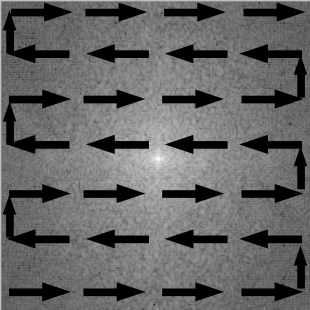
\includegraphics[width=2.5cm,height=2.5cm]{include/grp1/example_mask_kspace_with_arrows}
			
		} & \subfloat[\textcolor{black}{\scriptsize{} }]{\centering{}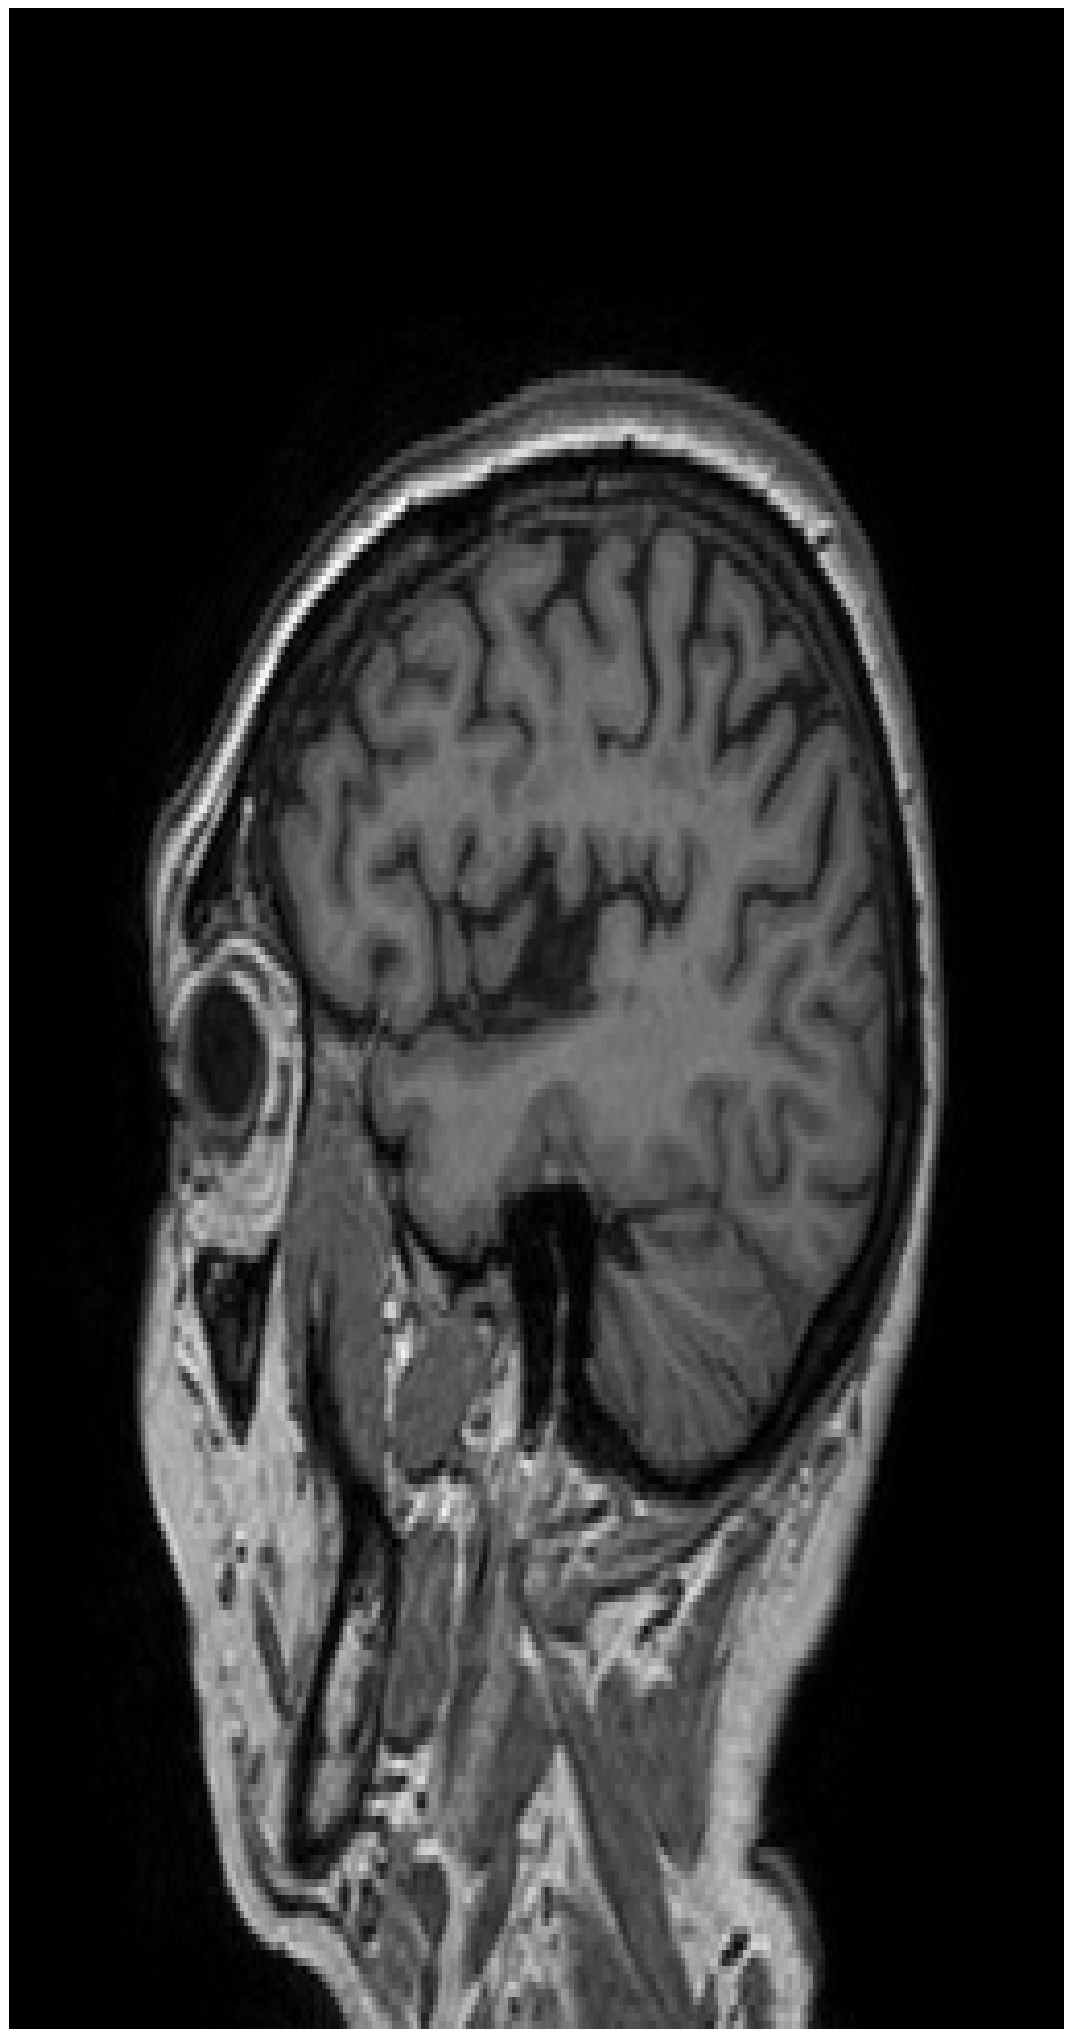
\includegraphics[width=2.5cm,height=2.5cm]{include/grp2/example_original.png}
		
	} & \subfloat[\textcolor{black}{\scriptsize{}}]{\centering{}
\includegraphics[width=2.5cm,height=2.5cm]{include/grp2/example_samplingMask4.png}\label{fig:pair_of_k_space_mri_mask}
	
} & \subfloat[\textcolor{black}{\scriptsize{}}]{\centering{}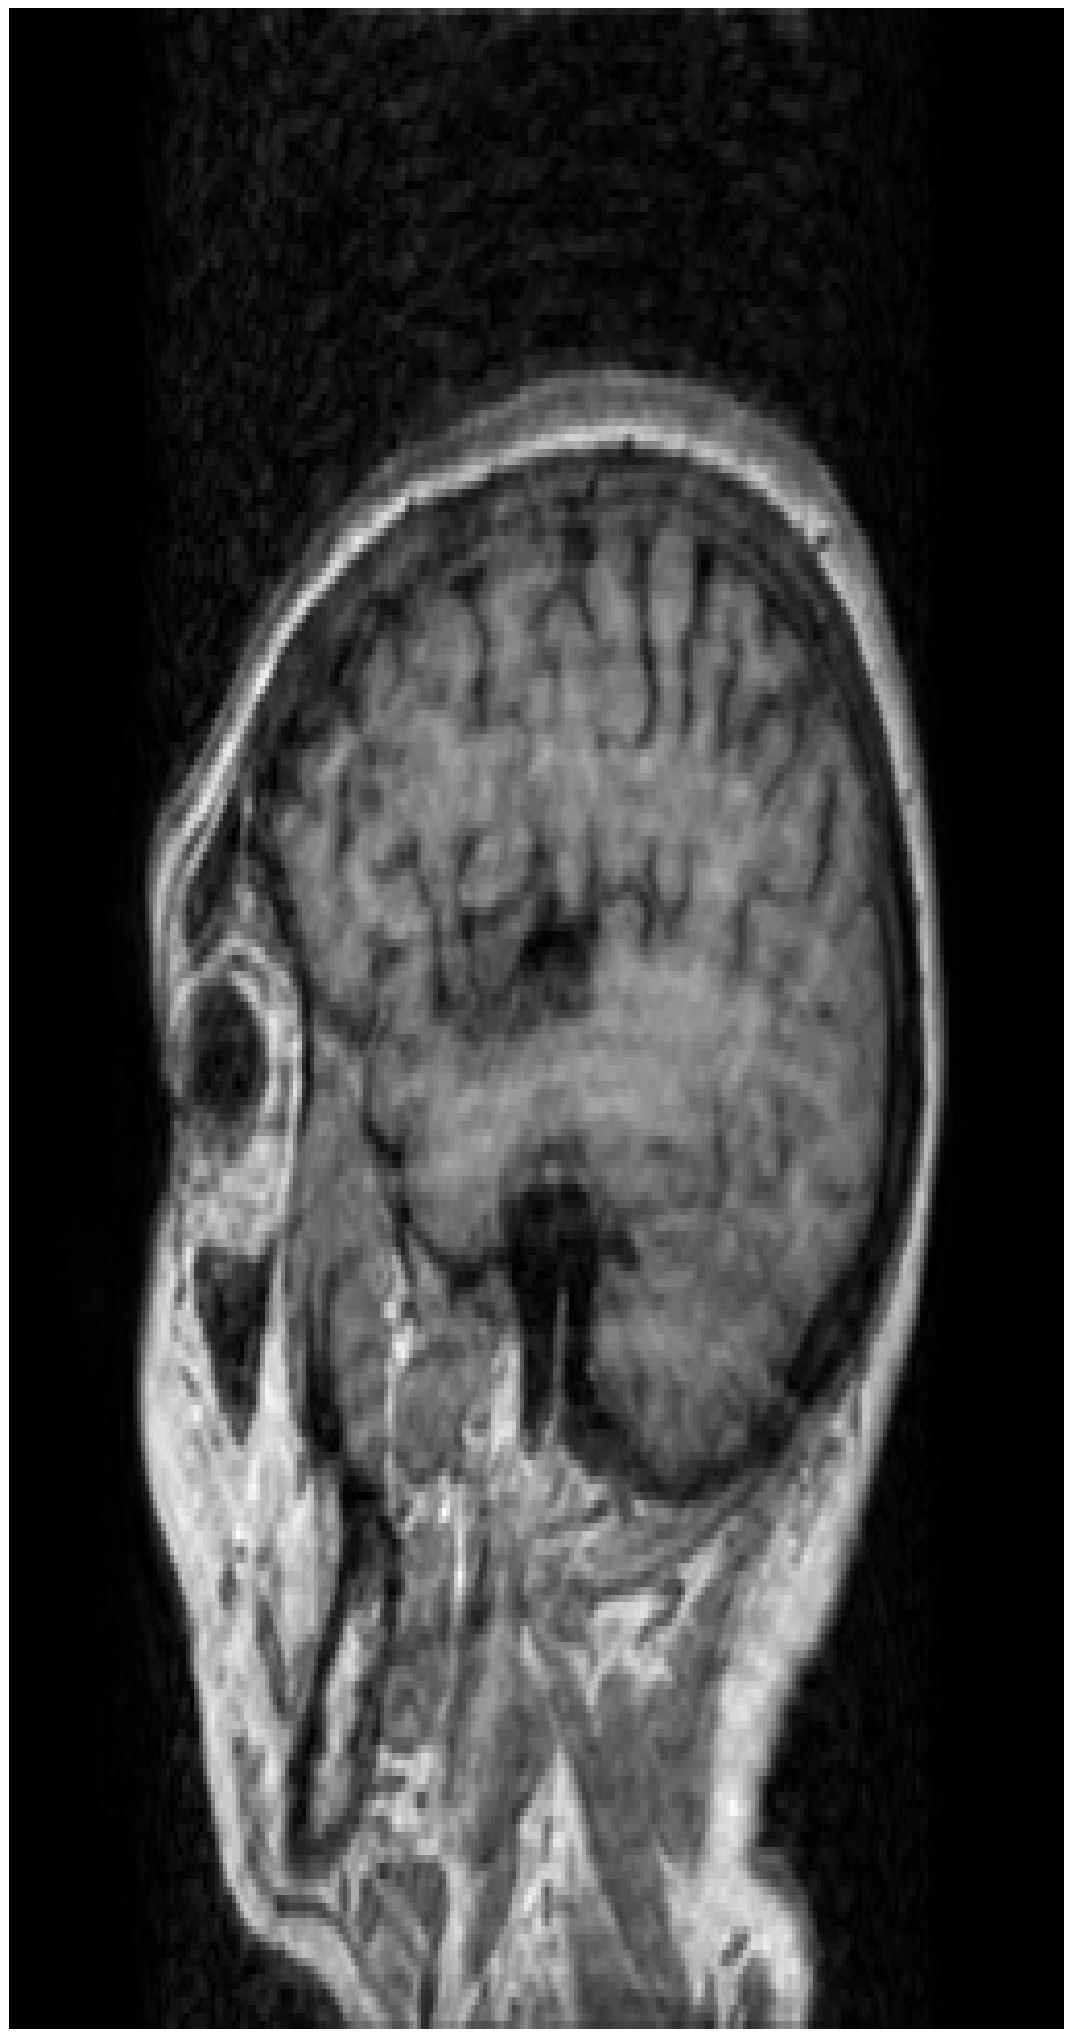
\includegraphics[width=2.5cm,height=2.5cm]{include/grp2/example_zeroPadding.png}\label{fig:pair_of_k_space_mri_example}
}\tabularnewline
\end{tabular}\caption{\textcolor{black}{\footnotesize{}{}(a) raw k-space: the
	arrows illustrate Cartesian sampling; (b) original; (c) sampling mask; (d) reconstructed}}
\label{fig:pair_of_k_space_mri} 
\end{figure}


Let $s_{p}=M_{p}\odot s_{0}$ denote the under-sampled k-space, where $\odot$ denotes element-wise multiplication and $M_{p}$ is the sampling mask. Given a model $f$, defined by the set of parameters $\Theta$, our goal is to estimate the missing k-space samples such that: 
\begin{equation}
\Theta=\arg\min_{\Theta}L(F^{H}f\left(s_{p};\Theta\right),\boldsymbol{u})
\end{equation}
where $L\left(\cdot\right)$ is a loss function. L2 loss is widely used for natural image reconstruction. However, as mentioned in~\cite{pathak2016context}, L2 minimization provides a blurry solution, resulting in a loss of fine details. In our case, where spatial frequencies in the form of k-space are considered, using this loss alone may be inappropriate, resulting in poor reconstruction. To address this problem, we propose 
the incorporation of an adversarial loss.

\subsection{K-space GAN}
We train our model using an adversarial strategy, as described in \cite{goodfellow2014generative,radford2015unsupervised}. 
This method is based on a generator $G$, which receives a noise \textbf{$z$}, sampled from a uniform distribution \textbf{$p_{u}\left(z\right)$}, as input and generates samples from the observed data distribution. A discriminator $D$ is trained to distinguish between true examples from the data and generated (``fake'') examples from $G.$ During the training process, we optimize $G$ to maximize the discriminator's probability of error. Simultaneously, $D$ is enhanced and provides more accurate predictions.

We assume that the true k-space samples, $s_{0}$, are drawn from the distribution $p_{r}\left(s_{0}\right)$. The optimization process can be defined by a two-players min-max value function $V(G,D)$:

\begin{equation}
\begin{split}
\min_{G}\max_{D}V(G,D) = \mathbb{E_{\mathrm{s_{0}\sim p_{r}\left(s_{0}\right)}}\mathrm{\log\left[D\left(s_{0}\right)\right]}}+
\\
\mathbb{E_{\mathrm{z\sim p_{u}\left(z\right)}}\mathrm{\log\left[1-D\left(G(z)\right)\right]}}
\end{split}
\end{equation}
%where $z$ is a noise drawn from a uniform distribution $p_{u}\left(z\right)$.
In equilibrium, the generator $G$ imitates the true data, which is in our case the missing k-space samples. The generator loss is a linear combination of L2 fidelity loss and an adversarial loss as follows:

\begin{equation}
\begin{aligned}L_{G}=\alpha\cdot E_{\mathrm{z\sim p_{u}\left(z\right)}}\mathrm{\log\left[1-D\left(F^{-1}\left(\hat{s}_{0}\right)\right)\right]}+\\
\beta\cdot||\left(1-M_{p}\right)\odot\left(\hat{s}_{0}-s_{0}\right)||_{2}^{2}
\end{aligned}
\end{equation}
where $\hat{s}_{0}$ is the estimated k-space and $\alpha=1,\,\beta=1$ are hyperparameters tuned by a cross-validation process.
We choose to use the Wasserstein distance as the GAN loss function (WGAN)~\cite{arjovsky2017wasserstein}, which improves the training stability and provides better reconstruction compared to the classic GAN loss we used in our preliminary work~\cite{shitrit2017accelerated}.

\subsection{System Architecture}
The proposed framework is illustrated in Figure~\ref{fig:system}.
\begin{figure}[H]
	\centering{}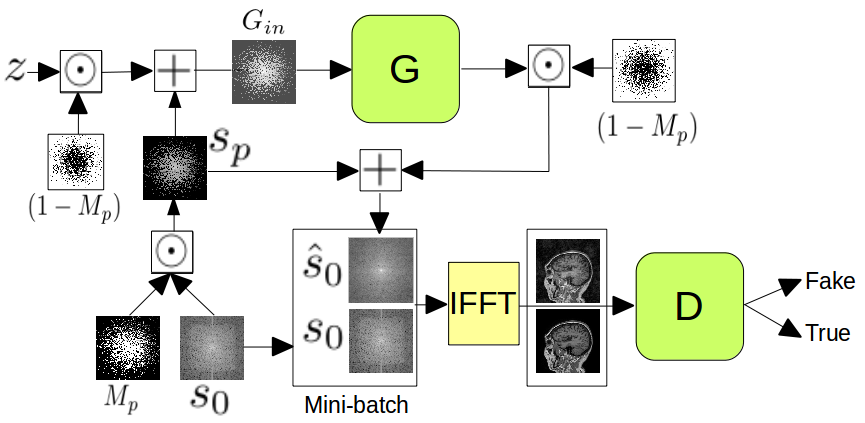
\includegraphics[width=12.0cm,height=4.0cm]{include/grp2/system_chart}\caption{\label{fig:system} \textcolor{black}{\footnotesize{}{}Framework
			architecture: $G$ and $D$ are the generator and discriminator networks,
			respectively. See text for details.}}
\end{figure}

The generator's input is a two-channel signal representing the real and the imaginary parts of the partially sampled k-space image, $s_{p}$. Each missing sample $\left(i,j\right)$ is initialized by uniform i.i.d. noise as follows: 
\begin{equation}
G_{in}\left(i,j\right)=s_{p_{i,j}}+\left(1-M_{p}\right)_{i,j}z_{i,j}
\end{equation}

$G$ estimates the missing k-space samples from a given samples and noise distribution $p_{u}\left(z\right)$. In order to utilize the remaining sampled data, $s_{p}$, and estimate only the missing samples we use a residual network \cite{he2016deep} as in \cite{Oktay2016}, such that:
\begin{equation}
\hat{s}_{0}=s_{p}+\left(1-M_{p}\right)\odot G_{out}
\end{equation}
where, $G_{out}$ is the generator output. The discriminator's two-channel (real and imaginary) input is either the reconstructed MR image obtained by IFFT of the generator's estimated or the true MR image obtained by IFFT of the original fully-sampled k-space data. By that, we are incorporating the IFFT into the network performing end-to-end optimization. The discriminator's output defines the WGAN loss.

We use a standard discriminator architecture, composed of convolutional layers, batch normalization, and leaky-ReLU as suggested in \cite{radford2015unsupervised}. For the generator, we compose a dedicated architecture, detailed in Section~\ref{experiments_section}. Both the discriminator and the generator inputs are two-channel image for the real and imaginary components. Figure~\ref{fig:architectures} illustrates the proposed architectures. During the training phase, $k_{d}$ discriminator update steps are carried out for every step of the generator. The training ends when the discriminator cannot accurately distinguish between the reconstructed (``fake'') and the true inputs.

%\vspace{-2.5cm}
\begin{figure*}[ht]
	\centering{}%
	\begin{tabular}{|c|}
		\hline 
		\subfloat[\textcolor{black}{\footnotesize{}Generator}]{\centering{}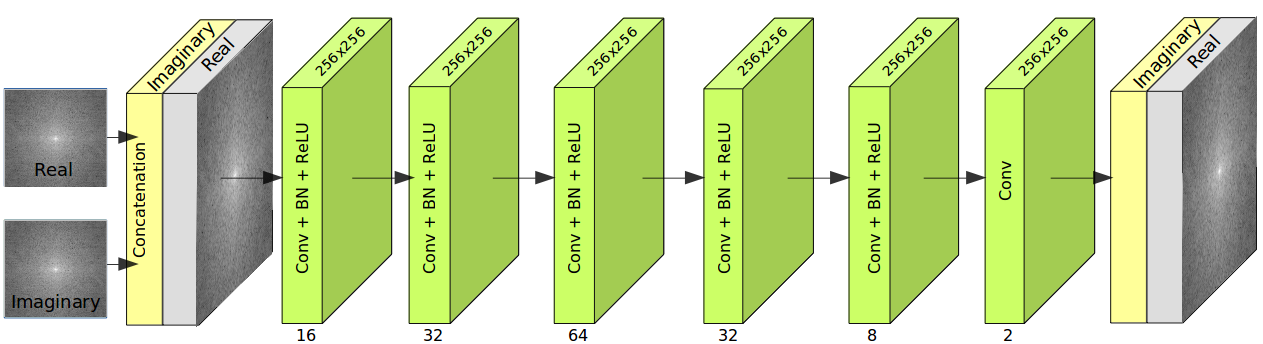
\includegraphics[width=11cm,height=2cm]{include/grp2/generator_arch} 
			
		}\tabularnewline
		\hline 
		\hline 

		\subfloat[\textcolor{black}{\footnotesize{}Discriminator}]{\centering{}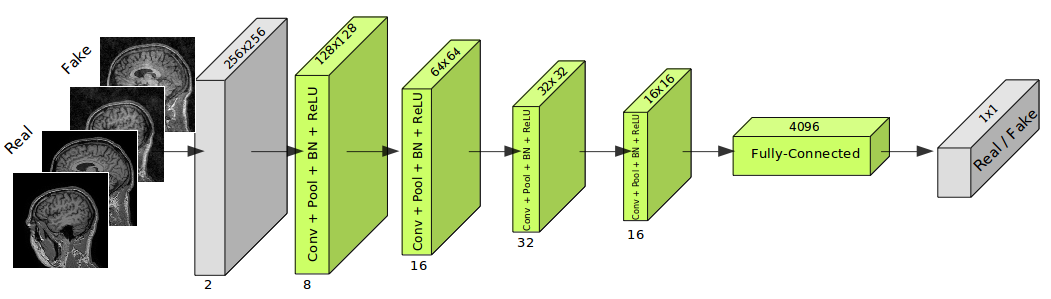
\includegraphics[width=11cm,height=2cm]{include/grp2/discrimonator_arch} 
			
		}\tabularnewline
		\hline 
	\end{tabular}\caption{\textcolor{black}{\footnotesize{}{}Networks architecture. Both the discriminator and the generator inputs are two-channel image for the real and imaginary components. The number above each layer represents the output channels. All convolutional kernels are $3\times3$.}}
\label{fig:architectures} 
\end{figure*}



%--------------------- Experiments --------------------%
\section{Experiments}\label{experiments_section}
\subsubsection*{\bf Data and sampling}
The training data consists of 500 3D brain MRI (T1-weighted) scans of different patients from the IXI dataset.\footnote{\url{http://brain-development.org/ixi-dataset/}} The data was acquired by three MR machines, Philips 1.5T, 3T and GE 1.5T using different imaging protocols.
From each 3D volume we extracted 93 2D saggital slices. All slices were interpolated to $256\times256$ pixels. We used $37.2k$ $(80\%)$ 2D slices for training and $9.3k$ $(20\%)$ for testing (100 3D volumes).
To create k-space images for training, inverse orthonormal
2D FFT was applied to the fully-sampled MR images. 
%Unlike our preliminary work~\cite{shitrit2017accelerated}, which employed a sampling mask along the phase axis alone; here, we perform k-space sampling using a 2D random Gaussian mask. By this, we exploit the sparsity in both phase and frequency dimensions and are therefore able to accommodate higher sampling factors (Figure~\ref{fig:sampling_masks}). MRI reconstruction is performed using 40\%, 25\%, and 16.6\% of the original k-space data.
We perform k-space sampling using a 2D random Gaussian mask. Thus, we exploit the sparsity in both phase and frequency dimensions and are therefore able to accommodate higher sampling factors (Figure~\ref{fig:sampling_masks}). MRI reconstruction is performed using 40\%, 25\%, and 16.6\% of the original k-space.

\subsubsection*{\bf Architecture}
The generator is composed of $5$ blocks of CONV-BatchNorm-ReLU, with output channels $16,32,64,32,8,$ respectively (see Figure~\ref{fig:architectures}). The last CONV layer is composed of two output channels for real and imaginary components. The discriminator is composed of $4$ blocks of CONV-Pool-BatchNorm-leaky-ReLU with output channels $8,16,32,16$ and one fully-connected layer. All CONV layers' kernel size is $3\times3$. All weights were initialized using Xavier \cite{glorot2010understanding}. We used the RMSprop~\cite{tieleman2012lecture} solver with a fixed learning rate of $5\mathrm{e}{-6}$ and set $k_{d}$ to 1.

\subsubsection*{\bf Comparisons}
We compared the proposed method reconstructions to those obtained by using a conventional compressed sensing method-CS-MRI \cite{lustig2007sparse} and zero-filling. In addition, we tested two other networks. To assess the use of an adversarial loss, we trained a k-space generator, with the same architecture as used in the proposed method, with only an L2 loss (CNN-L2). We also implemented the method proposed in~\cite{hyun2017deep} and constructed a network IM-CNN-L2, which is applied directly to the image space rather than the k-space. Specifically, as in~\cite{hyun2017deep}, we used the U-net architecture~\cite{ronneberger2015u} and applied an FFT on each of its output images to get an estimated k-space. The complete k-space is then recovered by integrating the estimated samples with the sampled raw data according to the sampling mask. The same sampling masks were used for all methods.

\subsubsection*{\bf Clinical usability}
To demonstrate the clinical usability of the reconstructed images we performed an extended validation, composed of anatomical quantitative measurements. In addition to the commonly used PSNR and Structure Similarity (SSIM) Index~\cite{wang2004image} metrics, we performed tissue segmentation and compared the results to those obtained by using the original fully-sampled images. The segmentation compatibility is measured in terms of Dice scores and Hausdorff distances.

%\vspace{-0.5cm}
\begin{figure}[H]
	\centering
	\setlength\tabcolsep{1.5pt}
	\begin{tabular}{ccc}
		\subfloat[{\scriptsize 40\%}]{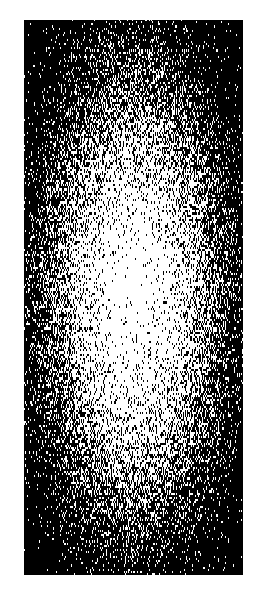
\includegraphics[width=3.0cm, height=3.0cm]{include/grp2/mask2}}
		& 
		\subfloat[{\scriptsize 25\%}]{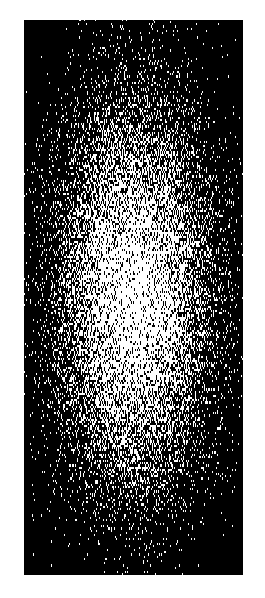
\includegraphics[width=3.0cm, height=3.0cm]{include/grp2/mask4}}
		&
		\subfloat[{\scriptsize 16.66\%}]{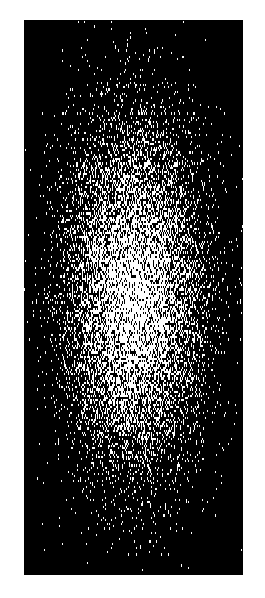
\includegraphics[width=3.0cm, height=3.0cm]{include/grp2/mask6}}
		\tabularnewline
		
	\end{tabular}\caption{{\footnotesize $2D$ Gaussian sampling masks}}
	\label{fig:sampling_masks}
\end{figure}

\subsection{PSNR and SSIM}
PSNR and SSIM are the most commonly used measures for evaluation of image reconstruction quality. PSNR measures the Mean Squared Error (MSE) between the fully-sampled MR image and the reconstructed image. SSIM quantifies the degradation caused by sampling artifacts based on pixels' inter-dependencies in the image.
Quantitative evaluation for both PSNR and SSIM is presented in~Table~\ref{tbl:PSNR_SSIM_NO_MASK}. The PSNR is calculated for the entire image without masking. Note that the proposed method outperforms the others. To support this claim, we also calculated the two-sample t-Test for the obtained scores. The differences are statistically significant (p-values~$<0.005$) for all pairwise comparisons between the results of our method and the others.

\begin{table*}[ht]
	\centering
	\resizebox{\textwidth}{!}{%
		\scriptsize
		\setlength\tabcolsep{2pt}
		\begin{tabular}{|c||c|c||c|c||c|c|}
			\hline 
			\textbf{PSNR/SSIM} & \multicolumn{2}{c||}{Factor 2.5 (40\%)} & \multicolumn{2}{c||}{Factor 4 (25\%)} & \multicolumn{2}{c|}{Factor 6 (16.66\%)}\tabularnewline
			\cline{2-6} 
			\textbf{Method}& PSNR & SSIM & PSNR & SSIM & PSNR & SSIM\tabularnewline
			\hline
			Zero-filled & 32.555{\tiny $\pm$}2.294 & 0.698{\tiny $\pm$}0.045 & 26.791{\tiny $\pm$}1.856 & 0.590{\tiny $\pm$}0.040 & 33.088{\tiny $\pm$}1.929 & 0.255{\tiny $\pm$}0.021\tabularnewline
			\hline 
			CS-MRI & 39.053{\tiny $\pm$}1.750 & 0.865{\tiny $\pm$}0.029 & 33.088{\tiny $\pm$}1.929 & 0.757{\tiny $\pm$}0.037 & 26.491{\tiny $\pm$}2.587 & 0.617{\tiny $\pm$}0.030\tabularnewline
			\hline
			IM-CNN-L2  & 39.663{\tiny $\pm$}1.934 & 0.884{\tiny $\pm$}0.030 & 35.042{\tiny $\pm$}2.042 & 0.796{\tiny $\pm$}0.036 & 28.134{\tiny $\pm$}2.181 & 0.606{\tiny $\pm$}0.023\tabularnewline
			\hline 
			CNN-L2 & 39.394{\tiny $\pm$}1.985 & 0.885{\tiny $\pm$}0.030 & 33.829{\tiny $\pm$}2.034 & 0.749{\tiny $\pm$}0.043 & 31.403{\tiny $\pm$}2.040 & 0.682{\tiny $\pm$}0.042\tabularnewline
			\hline 
			\textbf{Proposed} & \textbf{40.211{\tiny $\pm$}1.902} & \textbf{0.917{\tiny $\pm$}0.019} & \textbf{35.133{\tiny $\pm$}1.870} & \textbf{0.818{\tiny $\pm$}0.034} & \textbf{32.040{\tiny $\pm$}2.110} & \textbf{0.726{\tiny $\pm$}0.038}\tabularnewline
			\hline 
		\end{tabular}
	}
	\caption{\textcolor{black}{\footnotesize{}{}PSNR and SSIM for different sampling factors}{\footnotesize{}\label{tbl:PSNR_SSIM_NO_MASK}}}
\end{table*}


%\begin{table*}[ht]
%	\centering{}
%	\begin{tabular}{|c||c||c||c|}
%		\hline 
%		\textbf{PSNR} & \multicolumn{1}{c||}{\multirow{2}{*}{Factor 2.5 (40\%)}} & \multicolumn{1}{c||}{\multirow{2}{*}{Factor 4 (25\%)}} & \multicolumn{1}{c|}{\multirow{2}{*}{Factor 6 (16.66\%)}} \tabularnewline
%		\textbf{Method} & \multicolumn{1}{c||}{} & \multicolumn{1}{c||}{} & \multicolumn{1}{c|}{} \tabularnewline \cline{1-4}
%		
%		Zero-filled         &32.555~$\pm$~2.294  &26.791~$\pm$~1.856 &16.781~$\pm$~1.737\tabularnewline
%		CS-MRI              &39.053~$\pm$~1.750  &33.088~$\pm$~1.929 &26.491~$\pm$~2.587\tabularnewline
%		IM-CNN-L2           &39.663~$\pm$~1.934  &35.042~$\pm$~2.042 &28.134~$\pm$~2.181\tabularnewline
%		CNN-L2              &39.394~$\pm$~1.985  &33.829~$\pm$~2.034 &31.403~$\pm$~2.040\tabularnewline
%		\textbf{Proposed}   &\textbf{40.211~$\pm$~1.902}  &\textbf{35.133~$\pm$~1.870}   &\textbf{32.040~$\pm$~2.110}\tabularnewline
%		\hline 
%	\end{tabular}\caption{\textcolor{black}{\footnotesize{}{}Error in PSNR, without masking}{\footnotesize{}\label{tbl:PSNR_NO_MASK}}}
%\end{table*}
%
%
%\begin{table*}[ht]
%	\centering{}
%	\begin{tabular}{|c||c||c||c|}
%		\hline 
%		\textbf{SSIM} & \multicolumn{1}{c||}{\multirow{2}{*}{Factor 2.5 (40\%)}} & \multicolumn{1}{c||}{\multirow{2}{*}{Factor 4 (25\%)}} & \multicolumn{1}{c|}{\multirow{2}{*}{Factor 6 (16.66\%)}} \tabularnewline
%		\textbf{Method} & \multicolumn{1}{c||}{} & \multicolumn{1}{c||}{} & \multicolumn{1}{c|}{} \tabularnewline \cline{1-4}
%		
%		Zero-filled         &0.698~$\pm$~0.0452  &0.590~$\pm$~0.040   &0.255~$\pm$~0.021\tabularnewline
%		CS-MRI              &0.865~$\pm$~0.029  &0.757~$\pm$~0.037   &0.617~$\pm$~0.030\tabularnewline
%		IM-CNN-L2           &0.884~$\pm$~0.030  &0.796~$\pm$~0.036   &0.606~$\pm$~0.023\tabularnewline
%		CNN-L2              &0.885~$\pm$~0.030  &0.749~$\pm$~0.043   &0.682~$\pm$~0.042\tabularnewline
%		\textbf{Proposed}   &\textbf{0.917~$\pm$~0.019}  &\textbf{0.818~$\pm$~0.034}   &\textbf{0.726~$\pm$~0.038}\tabularnewline
%		\hline 
%	\end{tabular}\caption{\textcolor{black}{\footnotesize{}{}SSIM for different sampling factors}{\footnotesize{}\label{tbl:SSIM_NO_MASK}}}
%\end{table*}

%\vspace{-0.5cm}
%\begin{figure}[H]
%\centering
%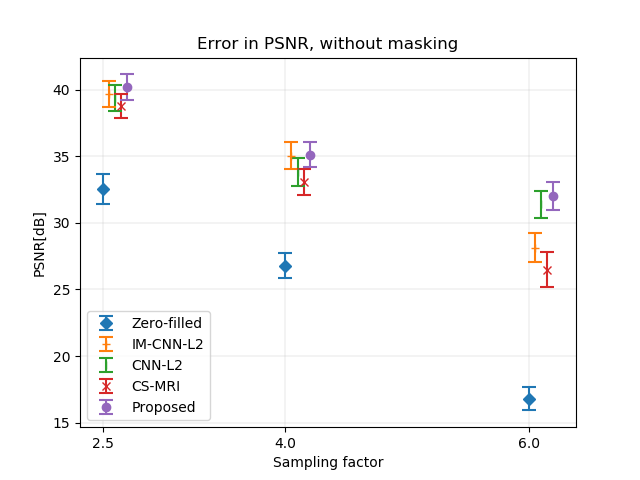
\includegraphics[width=1\linewidth]{include/grp2/error_psnr_errorbar}
%\caption{PSNR without masking error-bar}
%\label{fig:psnr_errorbar}
%\end{figure}

An additional validation of our model is performed by calculating the PSNR measure on different brain tissues. We applied the commonly used FAST~\cite{zhang2001segmentation} image segmentation algorithm on the original fully-sampled MR image and then used it for calculating the masked-PSNR on gray matter (GM), white matter (WM), and the Cerebrospinal Fluid (CSF). Results are presented in~Table~\ref{tbl:PSNR_WITH_MASK}. 
The differences are statistically significant with p-values~$<0.0005$ for CS-MRI and zero-filled for sampling factors 2.5 and 4, and also for IM-CNN-L2 with p-values~$<0.0001$ for sampling factor 6.

\begin{table*}[ht]
	\centering
	\resizebox{\textwidth}{!}{%
		\scriptsize
		\setlength\tabcolsep{2pt}
		\begin{tabular}{|c||c|c|c||c|c|c||c|c|c|}
			\hline 
			\textbf{PSNR} & \multicolumn{3}{c||}{Factor 2.5 (40\%)} & \multicolumn{3}{c||}{Factor 4 (25\%)} & \multicolumn{3}{c|}{Factor 6 (16.66\%)}\tabularnewline
			\cline{2-10} 
			\textbf{Method}& White & Gray & CSF & White & Gray & CSF & White & Gray & CSF\tabularnewline
			\hline 
			Zero-filled & 41.49{\tiny $\pm$}3.48 & 36.73{\tiny $\pm$}3.32 & 38.54{\tiny $\pm$}2.45 & 37.27{\tiny $\pm$}2.18 & 34.37{\tiny $\pm$}2.52 & 36.36{\tiny $\pm$}1.87 & 24.88{\tiny $\pm$}1.62 & 24.98{\tiny $\pm$}1.91 & 29.33{\tiny $\pm$}2.08\tabularnewline
			\hline 
			CS-MRI & 44.37{\tiny $\pm$}4.20 & 40.04{\tiny $\pm$}3.84 & 40.74{\tiny $\pm$}3.16 & 41.65{\tiny $\pm$}3.12 & 37.24{\tiny $\pm$}2.99 & 39.11{\tiny $\pm$}2.43 & 35.59{\tiny $\pm$}3.15 & 33.11{\tiny $\pm$}2.91 & 36.64{\tiny $\pm$}2.26\tabularnewline
			\hline
%			IM-CNN-L2 & 42.99{\tiny $\pm$}3.81 & 38.82{\tiny $\pm$}3.69 & 39.92{\tiny $\pm$}3.11 & 40.57{\tiny $\pm$}2.66 & 37.10{\tiny $\pm$}2.90 & 38.47{\tiny $\pm$}2.31 & 34.74{\tiny $\pm$}2.89 & 31.49{\tiny $\pm$}2.43 & 33.71{\tiny $\pm$}1.80\tabularnewline
			IM-CNN-L2  & 45.66{\tiny $\pm$}4.60 & 41.06{\tiny $\pm$}4.27 & 41.51{\tiny $\pm$}3.58 & 43.47{\tiny $\pm$}3.22 & 39.36{\tiny $\pm$}3.19 & 40.16{\tiny $\pm$}2.51 & 37.34{\tiny $\pm$}3.19 & 34.18{\tiny $\pm$}2.85 & 36.61{\tiny $\pm$}2.10\tabularnewline
			\hline  
			CNN-L2 & 45.72{\tiny $\pm$}4.70 & 41.59{\tiny $\pm$}4.16 & 41.68{\tiny $\pm$}3.69 & 43.26{\tiny $\pm$}2.95 & 40.15{\tiny $\pm$}3.15 & 40.24{\tiny $\pm$}2.47 & 41.11{\tiny $\pm$}2.48 & 39.27{\tiny $\pm$}2.65 & 39.10{\tiny $\pm$}1.93\tabularnewline
			\hline 
			\textbf{Proposed} & \textbf{46.20{\tiny $\pm$}4.77} & \textbf{41.94{\tiny $\pm$}4.34} & \textbf{41.61{\tiny $\pm$}2.45} & \textbf{43.85{\tiny $\pm$}3.16} & \textbf{40.11{\tiny $\pm$}3.25} & \textbf{40.49{\tiny $\pm$}2.57} & \textbf{41.91{\tiny $\pm$}2.77} & \textbf{39.01{\tiny $\pm$}2.88} & \textbf{39.36{\tiny $\pm$}2.17}\tabularnewline
			\hline 
		\end{tabular}
	}
	\caption{\textcolor{black}{\footnotesize{}{}Error in PSNR, with masking}{\footnotesize{}\label{tbl:PSNR_WITH_MASK}}}
\end{table*}


%We next used SSIM, which is a full reference metric, and is considered a perception-based model, to measure the similarity between the original fully-sampled images and the reconstructed ones.
%It quantifies the degradation caused by sampling artifacts based on pixels' inter-dependencies in the image. 
%SSIM scores for different sampling factors, for all methods compared, are presented in~Table~\ref{tbl:SSIM_NO_MASK}. The advantage of our method is clearly shown. All pairwise comparisons between the results obtained by our method and the others are statistically significant (p-values~$<0.0001$) for all sampling factors.

%\begin{table*}[ht]
%	\centering{}
%	\begin{tabular}{|c||c||c||c|}
%		\hline 
%		\textbf{SSIM} & \multicolumn{1}{c||}{\multirow{2}{*}{Factor 2.5 (40\%)}} & \multicolumn{1}{c||}{\multirow{2}{*}{Factor 4 (25\%)}} & \multicolumn{1}{c|}{\multirow{2}{*}{Factor 6 (16.66\%)}} \tabularnewline
%		\textbf{Method} & \multicolumn{1}{c||}{} & \multicolumn{1}{c||}{} & \multicolumn{1}{c|}{} \tabularnewline \cline{1-4}
%		
%		Zero-filled         &0.698~$\pm$~0.0452  &0.590~$\pm$~0.040   &0.255~$\pm$~0.021\tabularnewline
%		CS-MRI              &0.865~$\pm$~0.029  &0.757~$\pm$~0.037   &0.617~$\pm$~0.030\tabularnewline
%		IM-CNN-L2           &0.884~$\pm$~0.030  &0.796~$\pm$~0.036   &0.606~$\pm$~0.023\tabularnewline
%		CNN-L2              &0.885~$\pm$~0.030  &0.749~$\pm$~0.043   &0.682~$\pm$~0.042\tabularnewline
%		\textbf{Proposed}   &\textbf{0.917~$\pm$~0.019}  &\textbf{0.818~$\pm$~0.034}   &\textbf{0.726~$\pm$~0.038}\tabularnewline
%		\hline 
%	\end{tabular}\caption{\textcolor{black}{\footnotesize{}{}SSIM for different sampling factors}{\footnotesize{}\label{tbl:SSIM_NO_MASK}}}
%\end{table*}

While PSNR and SSIM are widely used, these measures are not sensitive enough to differences in fine details and complex anatomical structure topologies. For example, a model can provide a good reconstruction in the sense of PSNR, yet with blurry edges and therefore loss of high frequency information. This may significantly affect diagnostic usability. We, therefore, further compare segmentation quality between the fully-sampled and the reconstruction images. Results of the analysis obtained for our method and all others are presented next.

\subsection{Brain Extraction - Skull Stripping}
%Brain extraction (skull stripping) is an algorithm that delineates the brain boundary (Figure~ \ref{fig:brain_extraction}). It is a necessary preliminary step for brain analysis algorithms.
%We examine the different reconstruction methods by applying the Brain Extraction Tool (BET) \cite{smith2002fast} to both MR reconstructed and original (fully-sampled) images. Compatibility of the skull stripping results between the original and the generated datasets is measured via the Modified Hausdorff Distance (MHD)~\cite{dubuisson1994modified}, defined as follows.
%
%Let $C_1,C_2\in R^2$ denote the brain boundaries extracted by the BET algorithm, using the original and the reconstructed scans, respectively. The MHD between $C_1$ and $C_2$ is:
%
%\begin{equation}
%\begin{array}{cc}
%MHD(C_1,C_2) = 0.5 \left[{|C_1|^{-1} \sum_{\sigma_{1}\in C_1}^{}d(\sigma_1,C_2) + |C_2|^{-1} \sum_{\sigma_{2}\in C_2}^{}d(\sigma_2,C_1)}\right] \\
%d(\sigma_1,C_2) = \underset{\sigma_{2}\in C_{2}}{\min}||\sigma_1-\sigma_2|| \\
%d(\sigma_2,C_1) = \underset{\sigma_{1}\in C_{1}}{\min}||\sigma_2-\sigma_1||
%\end{array}
%\end{equation}
%
%where $\sigma_1,\sigma_2$ are points on the contours $C_1,C_2$, respectively (Figure~\ref{fig:brain_extraction}.c) and $|C_i|,~i=1,2$, are the respective cardinalities. MHD values for all tested methods and sampling ratios are presented in~Table~\ref{tbl:MHD}. The MHD results obtained by our methods are better than all others and are significant (p-values~$<0.0001$) for CS-MRI and zero-filled.

Brain extraction (skull stripping) is an algorithm that delineates the brain boundaries. It is a necessary preliminary step for brain analysis algorithms.
We examine the different reconstruction methods by applying the Brain Extraction Tool (BET) \cite{smith2002fast} to both MR reconstructed and original (fully-sampled) images. Compatibility of the skull stripping results between the original and the generated datasets is measured via the Modified Hausdorff Distance (MHD)~\cite{dubuisson1994modified}. 
%defined as follows.
%
%Let $C_1,C_2\in R^2$ denote the brain boundaries extracted by the BET algorithm, using the original and the reconstructed scans, respectively. The MHD between $C_1$ and $C_2$ is:
%
%\begin{equation}
%\begin{array}{cc}
%MHD(C_1,C_2) = 0.5 \left[{|C_1|^{-1} \sum_{\sigma_{1}\in C_1}^{}d(\sigma_1,C_2) + |C_2|^{-1} \sum_{\sigma_{2}\in C_2}^{}d(\sigma_2,C_1)}\right] \\
%d(\sigma_1,C_2) = \underset{\sigma_{2}\in C_{2}}{\min}||\sigma_1-\sigma_2|| \\
%d(\sigma_2,C_1) = \underset{\sigma_{1}\in C_{1}}{\min}||\sigma_2-\sigma_1||
%\end{array}
%\end{equation}
%
%where $\sigma_1,\sigma_2$ are points on the contours $C_1,C_2$, respectively (Figure~\ref{fig:brain_extraction}.c) and $|C_i|,~i=1,2$, are the respective cardinalities.
MHD values for all tested methods and sampling ratios are presented in~Table~\ref{tbl:MHD}. The MHD scores obtained by our methods are better than all others and the differences are statistically significant (p-values~$<0.0001$) for CS-MRI and zero-filled.

\begin{table*}[ht]
	\centering{}
	\begin{tabular}{|c||c||c||c|}
		\hline 
		\textbf{MHD} & \multicolumn{1}{c||}{\multirow{2}{*}{Factor 2.5 (40\%)}} & \multicolumn{1}{c||}{\multirow{2}{*}{Factor 4 (25\%)}} & \multicolumn{1}{c|}{\multirow{2}{*}{Factor 6 (16.66\%)}} \tabularnewline
		\textbf{Method} & \multicolumn{1}{c||}{} & \multicolumn{1}{c||}{} & \multicolumn{1}{c|}{} \tabularnewline \cline{1-4}
				
		Zero-filled         &1.111~$\pm$~0.563  &2.617~$\pm$~1.214   &3.121~$\pm$~1.279\tabularnewline
		CS-MRI              &0.701~$\pm$~0.511  &1.447~$\pm$~1.027   &3.114~$\pm$~1.617\tabularnewline
%		IM-CNN-L2           &0.654~$\pm$~0.414  &0.878~$\pm$~0.548   &2.760~$\pm$~1.748\tabularnewline
		IM-CNN-L2           &0.541~$\pm$~0.388  &0.724~$\pm$~0.394   &1.902~$\pm$~1.437\tabularnewline
		CNN-L2              &0.420~$\pm$~0.270  &0.715~$\pm$~0.561   &1.083~$\pm$~1.052\tabularnewline
		\textbf{Proposed}   &\textbf{0.391~$\pm$~0.250}  &\textbf{0.617~$\pm$~0.306}   &\textbf{1.050~$\pm$~1.033}\tabularnewline
		\hline 
	\end{tabular}\caption{\textcolor{black}{\footnotesize{}{}MHD - brain extraction}{\footnotesize{}\label{tbl:MHD}}}
\end{table*}


%\begin{figure}[H]
%	\centering
%	\begin{tabular}{ccc}
%	\subfloat[\footnotesize MR image]{\includegraphics[width=2cm, height=2.2cm]{include/grp2/skull_stripping}} 
%	& 
%	\subfloat[\footnotesize Brain extraction]{\includegraphics[width=2cm, height=2.2cm]{include/grp2/skull_stripping_brain}}
%	&
%	\subfloat[\footnotesize Hausdorff distance]{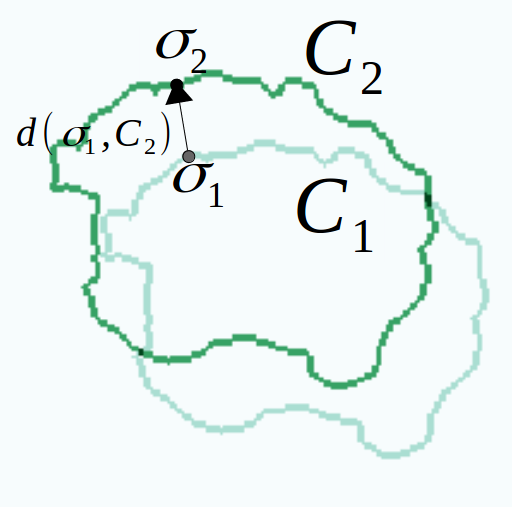
\includegraphics[width=2cm, height=2.2cm]{include/grp2/hausdorff}}
%	\tabularnewline
%
%	\end{tabular}\caption{{\footnotesize Example of brain extraction}}
%	\label{fig:brain_extraction}
%\end{figure}


\subsection{Brain Segmentation}
We next tested and compared segmentation quality by applying a brain tissue partitioning algorithm (FAST \cite{zhang2001segmentation}) to the reconstructed images. Segmentation results were compared to those obtained for the original fully-sampled scans. We believe that these comparisons are indicative of the diagnostic quality of the reconstructed MRIs as tissue segmentation (WM, GM, and CSF) plays a key role in clinical brain analysis.
%Segmentation compatibility demonstrate the quality of the proposed MRI reconstruction with respect to other methods. We create a reference segmentation by extracting the brain (using BET \cite{smith2002fast}) from the original fully-sampled image and perform a brain segmentation algorithm (FAST \cite{zhang2001segmentation}) on it. Then, we did the same process for all the reconstruction methods and compared the segmentation results.
We used the Dice score~\cite{dice1945measures} to measure the compatibility between the segments obtained for the original ($S_{\mbox{\tiny{REF}}}$) and the reconstructed ($S_{\mbox{\tiny{REC}}}$) images, defined as:
\begin{equation}
\begin{array}{c}
DICE(S_{\mbox{\tiny{REF}}}, S_{\mbox{\tiny{REC}}}) = 2\frac{S_{\mbox{\tiny{REF}}} \cap S_{\mbox{\tiny{REC}}}}{S_{\mbox{\tiny{REF}}} + S_{\mbox{\tiny{REC}}}}
\end{array}
\end{equation}
Dice scores are between zero and one, where one indicates complete overlap between the tested segments. Therefore, higher Dice scores imply higher compatibility between reconstructed and original images.
Dice scores for all tested methods and sampling factors are presented in~Table~\ref{tbl:DICE}. As for previous tests, our method achieves the best scores for all brain tissues and all sampling factors. Statistically significant values (p-values~$<0.0005$) were obtained for all methods using sampling factor of 2.5. In addition to the CS-MRI and zero-filled, the differences are statistically significant with p-values~$<0.0001$ for CNN-L2 using sampling factor 4 and for IM-CNN-L2 using sampling factor 6.

\begin{table*}[ht]
	\centering
	\resizebox{\textwidth}{!}{%
		\scriptsize
		\setlength\tabcolsep{2pt}
		\begin{tabular}{|c||c|c|c||c|c|c||c|c|c|}
			\hline 
			\textbf{DICE} & \multicolumn{3}{c||}{Factor 2.5 (40\%)} & \multicolumn{3}{c||}{Factor 4 (25\%)} & \multicolumn{3}{c|}{Factor 6 (16.66\%)}\tabularnewline
			\cline{2-10} 
			\textbf{Method}& White & Gray & CSF & White & Gray & CSF & White & Gray & CSF\tabularnewline
			\hline 
			Zero-filled & 0.882{\tiny $\pm$}0.08 & 0.826{\tiny $\pm$}0.05 & 0.796{\tiny $\pm$}0.05 & 0.718{\tiny $\pm$}0.10 & 0.644{\tiny $\pm$}0.05 & 0.627{\tiny $\pm$}0.05 & 0.599{\tiny $\pm$}0.12 & 0.466{\tiny $\pm$}0.07 & 0.050{\tiny $\pm$}0.06\tabularnewline
			\hline 
			CS-MRI & 0.942{\tiny $\pm$}0.05 & 0.910{\tiny $\pm$}0.03 & 0.868{\tiny $\pm$}0.03 & 0.871{\tiny $\pm$}0.10 & 0.805{\tiny $\pm$}0.08 & 0.770{\tiny $\pm$}0.05 & 0.708{\tiny $\pm$}0.14 & 0.639{\tiny $\pm$}0.08 & 0.621{\tiny $\pm$}0.07     \tabularnewline
			\hline 

%			IM-CNN-L2 & 0.908{\tiny $\pm$}0.04 & 0.863{\tiny $\pm$}0.03 & 0.839{\tiny $\pm$}0.03 & 0.832{\tiny $\pm$}0.05 & 0.754{\tiny $\pm$}0.03 & 0.754{\tiny $\pm$}0.03 & 0.695{\tiny $\pm$}0.11 & 0.590{\tiny $\pm$}0.06 & 0.560{\tiny $\pm$}0.06     \tabularnewline
%			\hline
			
			IM-CNN-L2  & 0.947{\tiny $\pm$}0.02 & 0.917{\tiny $\pm$}0.02 & 0.887{\tiny $\pm$}0.02 & 0.903{\tiny $\pm$}0.03 & 0.853{\tiny $\pm$}0.02 & 0.828{\tiny $\pm$}0.02 & 0.741{\tiny $\pm$}0.14 & 0.681{\tiny $\pm$}0.08 & 0.674{\tiny $\pm$}0.07     \tabularnewline
			\hline
			
			CNN-L2 & 0.948{\tiny $\pm$}0.02 & 0.919{\tiny $\pm$}0.02 & 0.891{\tiny $\pm$}0.02 & 0.888{\tiny $\pm$}0.06 & 0.836{\tiny $\pm$}0.04 & 0.813{\tiny $\pm$}0.03 & 0.836{\tiny $\pm$}0.09 & 0.770{\tiny $\pm$}0.06 & 0.747{\tiny $\pm$}0.06     \tabularnewline
			\hline
			
			\textbf{Proposed} & \textbf{0.954{\tiny $\pm$}0.01} & \textbf{0.928{\tiny $\pm$}0.02} & \textbf{0.900{\tiny $\pm$}0.002} & \textbf{0.903{\tiny $\pm$}0.06} & \textbf{0.858{\tiny $\pm$}0.04} & \textbf{0.833{\tiny $\pm$}0.03} & \textbf{0.851{\tiny $\pm$}0.09} & \textbf{0.789{\tiny $\pm$}0.06} & \textbf{0.767{\tiny $\pm$}0.06}     \tabularnewline
			\hline 
		\end{tabular}
	}
	
	\caption{\textcolor{black}{\footnotesize{}{}Segmentation Dice scores for different sampling ratios}{\footnotesize{}\label{tbl:DICE}}}
	
\end{table*}
MR reconstruction results for factor 6~(16.66\%) as well as their respective brain segmentation results are visually presented in Figure~\ref{fig:example_factor_6} for a single representative scan. The left-most column corresponds to the original image and columns 2-5 correspond to the reconstructed images using Zero-filled, CS-MRI, IM-CNN-L2, and the proposed method, respectively. The first row in Figure~\ref{fig:example_factor_6} presents a $2D$ slice of the original and the reconstructed MRIs. The second row presents the zoom-in of brain regions in the red frames shown in the first row. The third row presents the corresponding brain extraction. The fourth row presents the automatic tissue segmentation where, dark blue is used for WM, blue for GM and light blue for CSF. Note that MRIs reconstructed using the suggested adversarial method have stronger contrast and no significant aliasing or artifacts. In addition, the brain extraction and tissue segmentation results are more compatible with those obtained from the original fully-sampled MRIs. Additional examples of different cases, using sampling factors of 4~(25\%), and 2.5~(40\%) are shown in Figures~\ref{fig:example_factor_4},~\ref{fig:example_factor_2.5}, respectively.

% Examples factor 6
\begin{figure*}[ht]
	%	\begin{raggedright}
	\begin{raggedleft}
		%		\begin{tabular}{>{\centering}b{0.2cm}lcccc}
		\hspace*{-2cm} \begin{tabular}{cccccc}
			& \multicolumn{1}{c}{\footnotesize Original} & {\footnotesize Zero-filled} & {\footnotesize CS-MRI} & {\footnotesize IM-CNN-L2} & {\footnotesize Proposed}\tabularnewline
			\multirow{1}{0.05cm}[1.8cm]{\begin{turn}{90} {\footnotesize Reconstructed} \end{turn}} &
			
			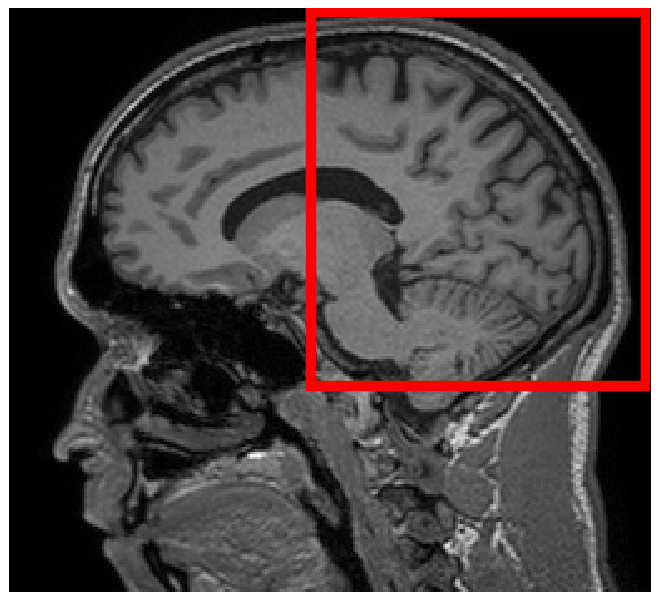
\includegraphics[width=2.5cm,height=2.5cm]{include/grp2/factor6/022-Guys-0701-T1/022-Guys-0701-T1_images__50} &
			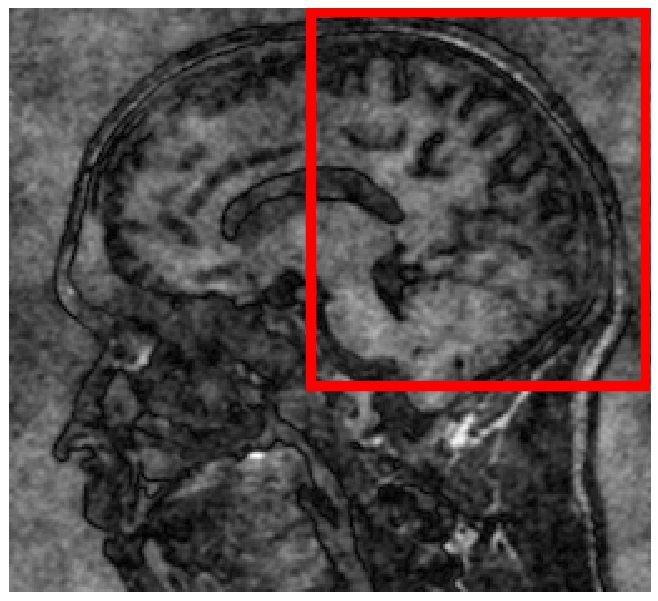
\includegraphics[width=2.5cm,height=2.5cm]{include/grp2/factor6/022-Guys-0701-T1/022-Guys-0701-T1_images__zeroPadding_50} & 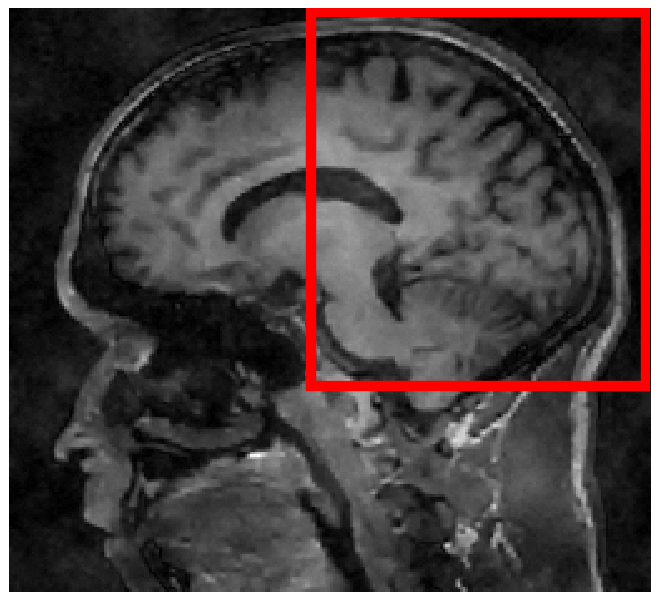
\includegraphics[width=2.5cm,height=2.5cm]{include/grp2/factor6/022-Guys-0701-T1/022-Guys-0701-T1_images__CS_50} & 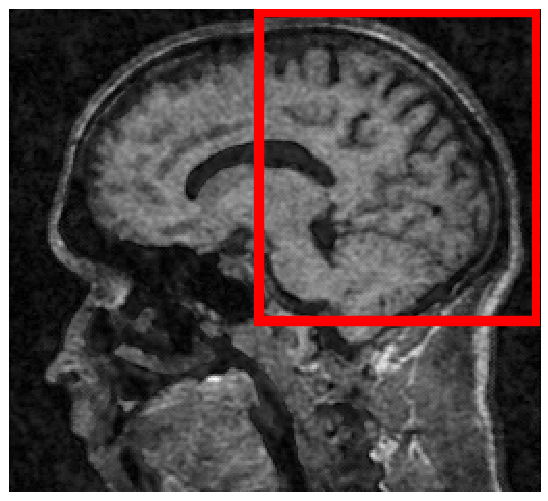
\includegraphics[width=2.5cm,height=2.5cm]{include/grp2/factor6/022-Guys-0701-T1/022-Guys-0701-T1_images__IMCNNL2TUNE_50} & 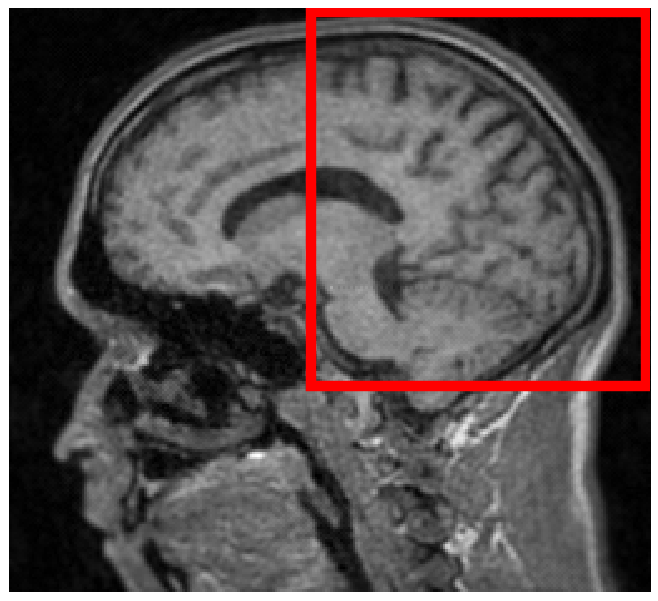
\includegraphics[width=2.5cm,height=2.5cm]{include/grp2/factor6/022-Guys-0701-T1/022-Guys-0701-T1_images__predict_50}
			
			\tabularnewline
			
			\multirow{1}{0.05cm}[1.3cm]{\begin{turn}{90} {\footnotesize Zoom in} \end{turn}} &
			
			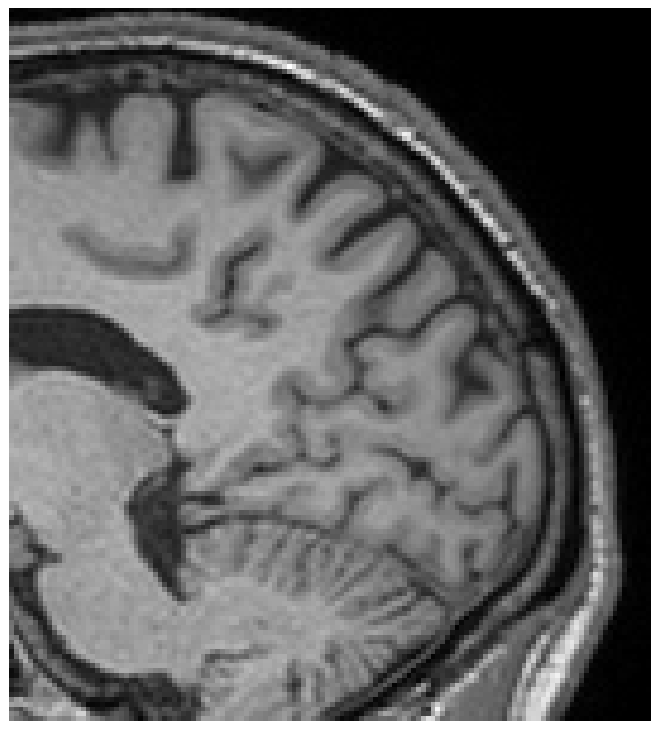
\includegraphics[width=2.5cm,height=2.5cm]{include/grp2/factor6/022-Guys-0701-T1/022-Guys-0701-T1_images__zoom_50} &
			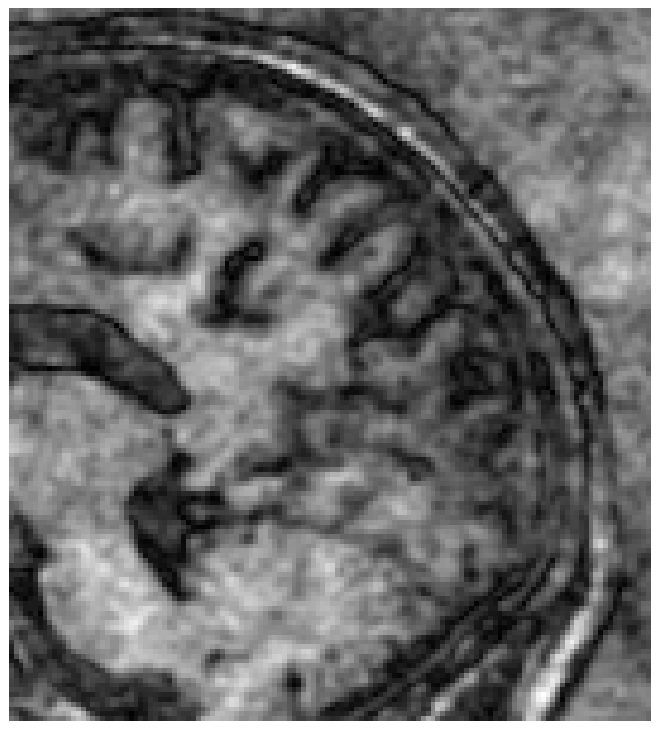
\includegraphics[width=2.5cm,height=2.5cm]{include/grp2/factor6/022-Guys-0701-T1/022-Guys-0701-T1_images__zeroPadding_zoom_50} & 
			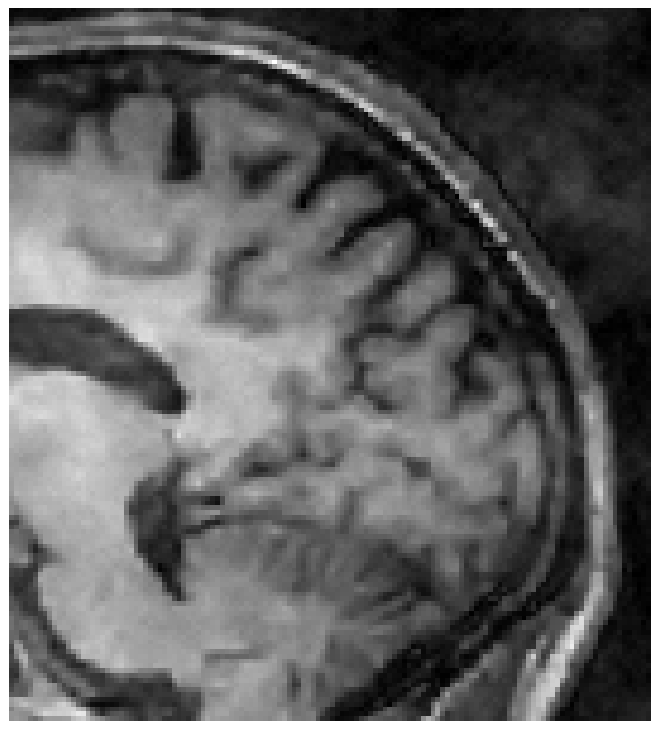
\includegraphics[width=2.5cm,height=2.5cm]{include/grp2/factor6/022-Guys-0701-T1/022-Guys-0701-T1_images__CS_zoom_50} & 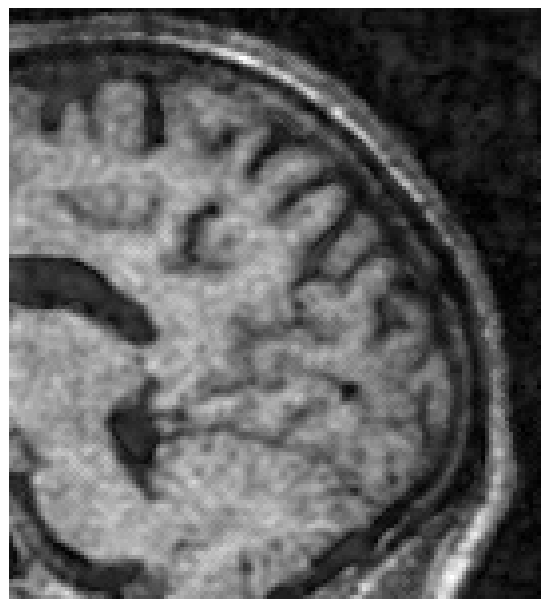
\includegraphics[width=2.5cm,height=2.5cm]{include/grp2/factor6/022-Guys-0701-T1/022-Guys-0701-T1_images__IMCNNL2TUNE_zoom_50} & 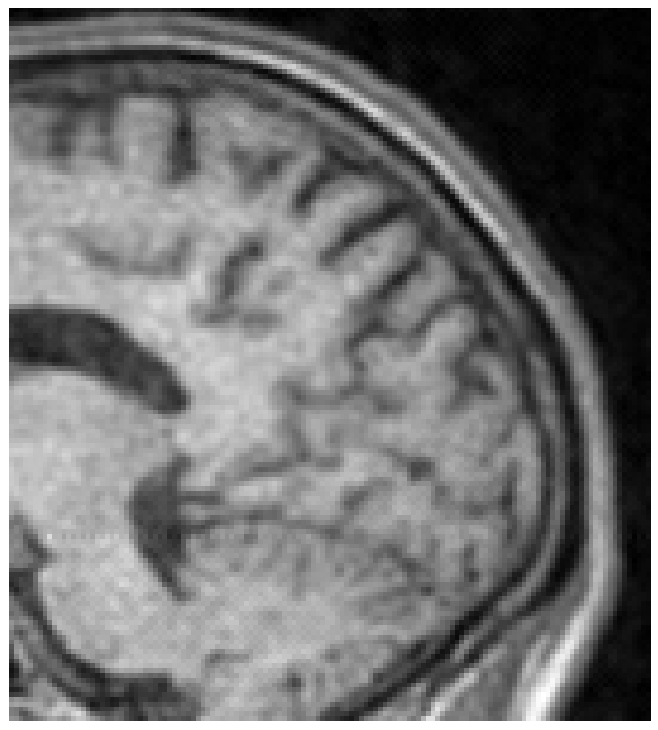
\includegraphics[width=2.5cm,height=2.5cm]{include/grp2/factor6/022-Guys-0701-T1/022-Guys-0701-T1_images__predict_zoom_50}
			
			\tabularnewline
			
			\multirow{2}{0.05cm}[1.4cm]{\begin{turn}{90} {\footnotesize Brain} \end{turn}} & 
			
			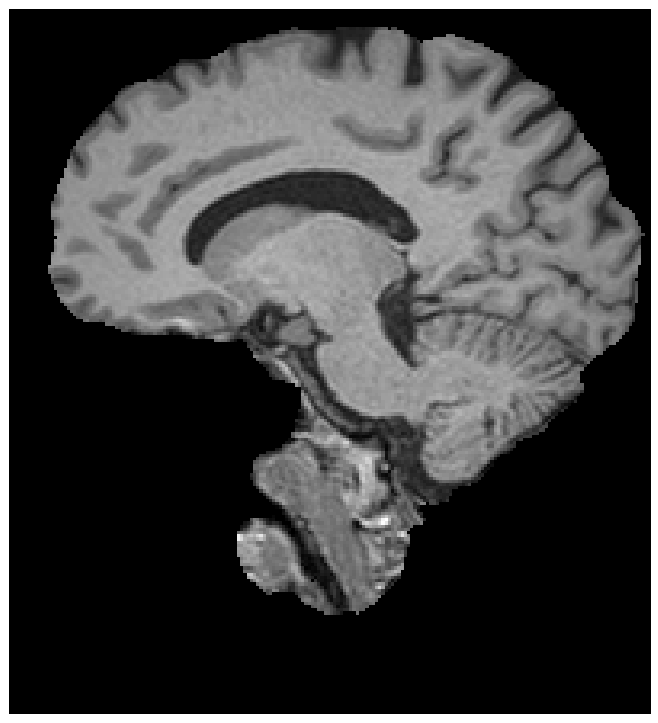
\includegraphics[width=2.5cm,height=2.5cm]{include/grp2/factor6/022-Guys-0701-T1/022-Guys-0701-T1_brains__50} &
			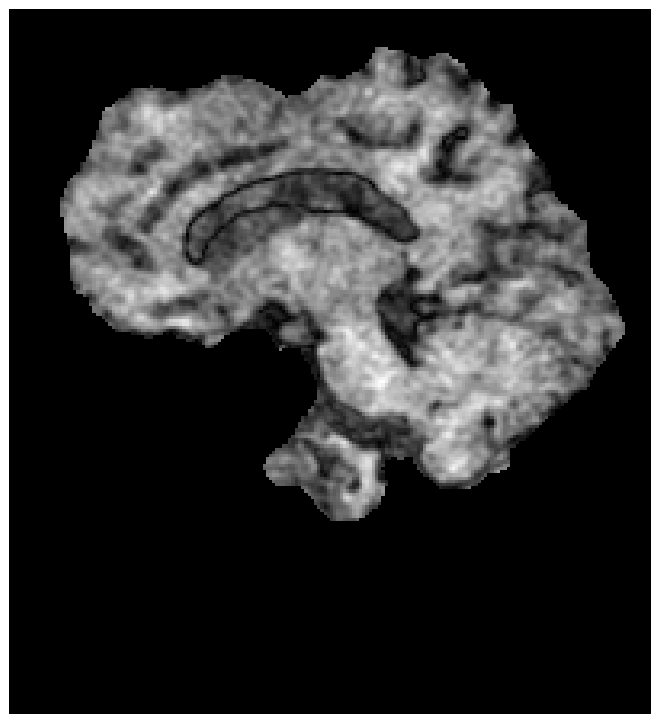
\includegraphics[width=2.5cm,height=2.5cm]{include/grp2/factor6/022-Guys-0701-T1/022-Guys-0701-T1_brains__zeroPadding_50} & 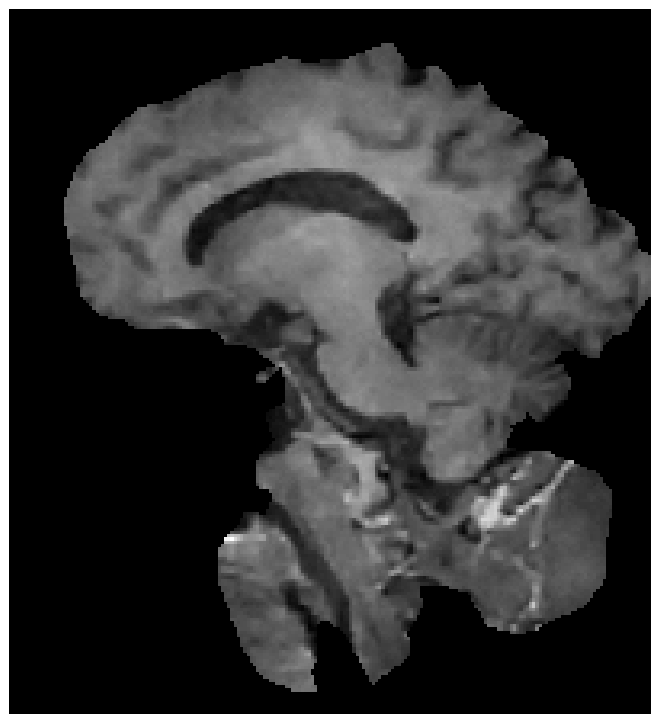
\includegraphics[width=2.5cm,height=2.5cm]{include/grp2/factor6/022-Guys-0701-T1/022-Guys-0701-T1_brains__CS_50} & 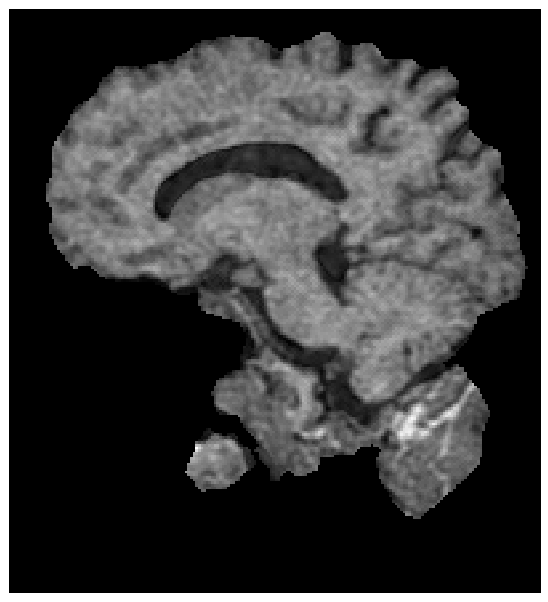
\includegraphics[width=2.5cm,height=2.5cm]{include/grp2/factor6/022-Guys-0701-T1/022-Guys-0701-T1_brains__IMCNNL2TUNE_50} & 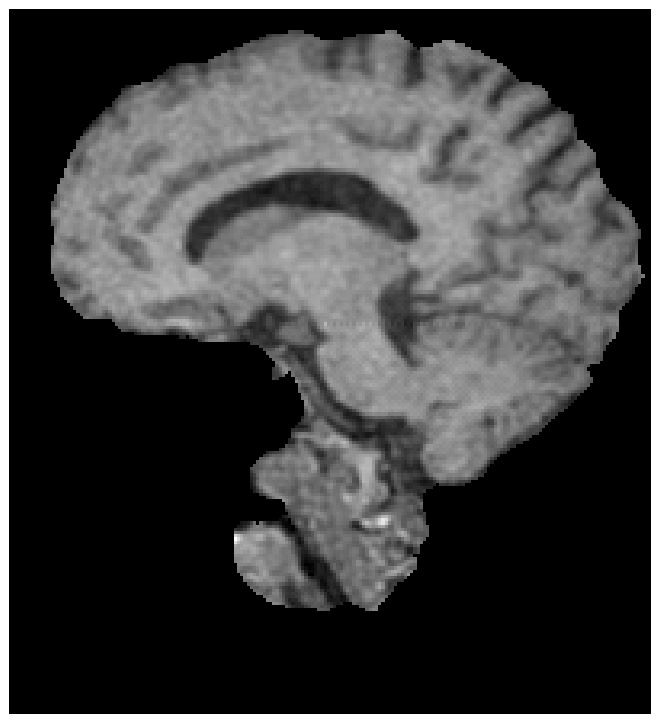
\includegraphics[width=2.5cm,height=2.5cm]{include/grp2/factor6/022-Guys-0701-T1/022-Guys-0701-T1_brains__predict_50}
			
			\tabularnewline
			
			\multirow{2}{0.05cm}[1.7cm]{\begin{turn}{90} {\footnotesize Segmentation} \end{turn}} &
			
			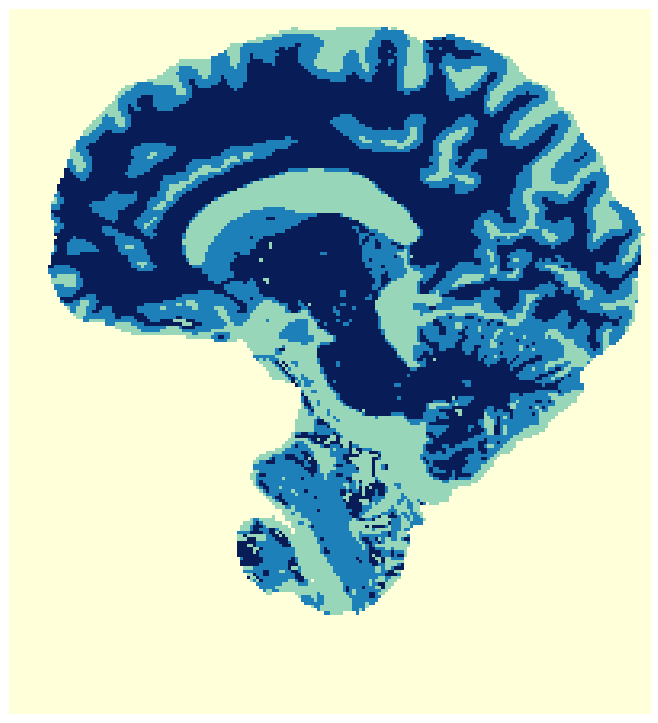
\includegraphics[width=2.5cm,height=2.5cm]{include/grp2/factor6/022-Guys-0701-T1/022-Guys-0701-T1_segs__50} &
			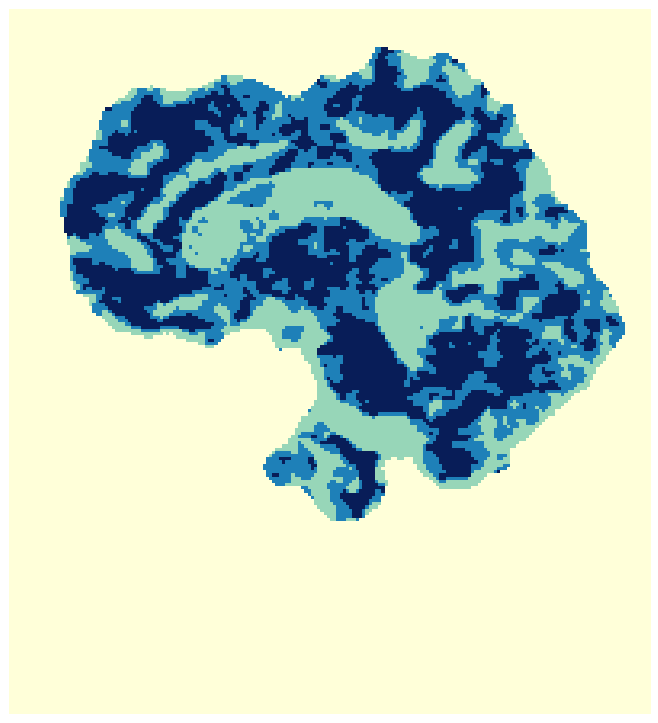
\includegraphics[width=2.5cm,height=2.5cm]{include/grp2/factor6/022-Guys-0701-T1/022-Guys-0701-T1_segs__zeroPadding_50} & 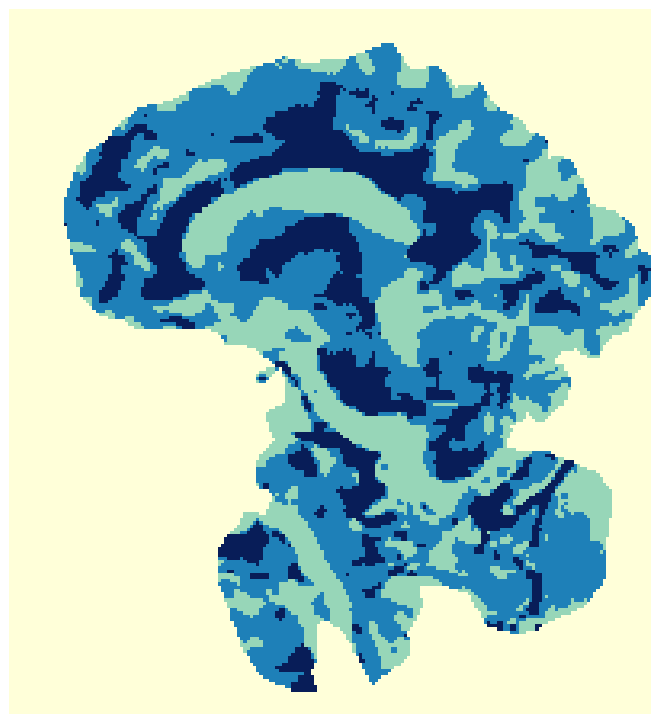
\includegraphics[width=2.5cm,height=2.5cm]{include/grp2/factor6/022-Guys-0701-T1/022-Guys-0701-T1_segs__CS_50} & 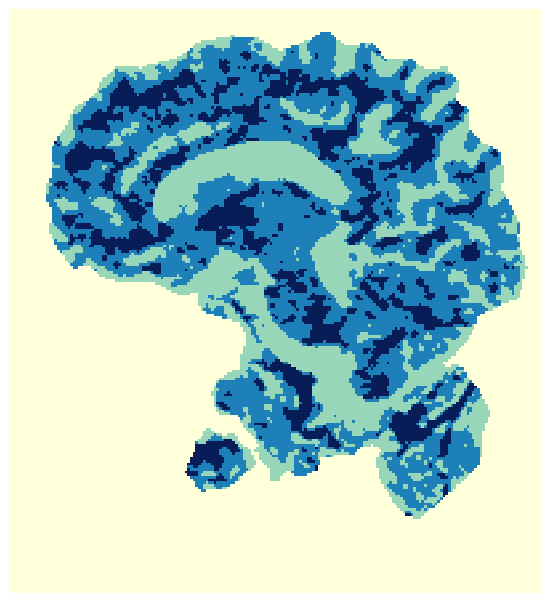
\includegraphics[width=2.5cm]{include/grp2/factor6/022-Guys-0701-T1/022-Guys-0701-T1_segs__IMCNNL2TUNE_50} & 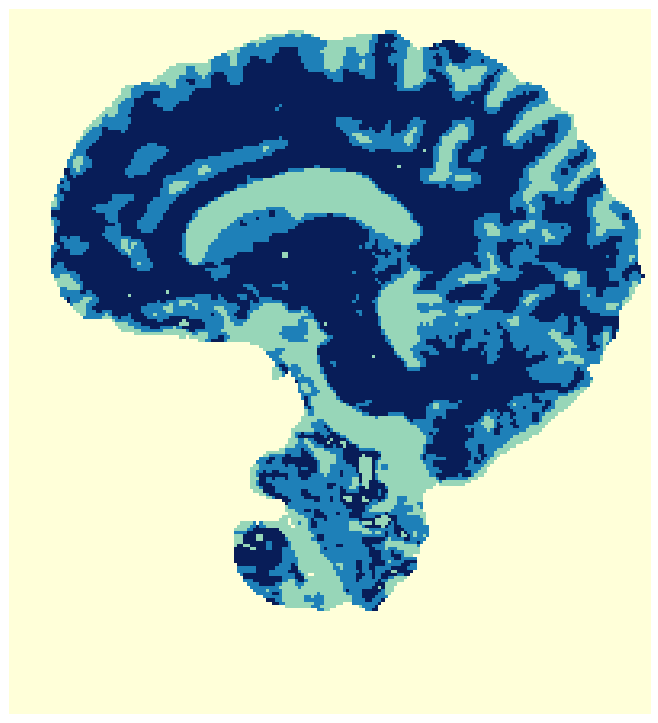
\includegraphics[width=2.5cm,height=2.5cm]{include/grp2/factor6/022-Guys-0701-T1/022-Guys-0701-T1_segs__predict_50}
			
			
		\end{tabular}
		\par\end{raggedleft}
	\raggedright{}\caption{\textcolor{black}{\footnotesize{}Examples of reconstructed MR images from under-sampled k-space - Factor 6.}}
	\label{fig:example_factor_6} 
\end{figure*}

%--------------------- CONCLUSIONS --------------------%
\section{Discussion}\label{conclusions_section}
The proposed deep learning framework for MRI reconstruction from highly under-sampled k-space (up to 16.66\%), can be used as the foundation of a real-time, software-only solution for MRI acceleration.
The inter-play between the generator and the discriminator plays a key role here. The generator is trained directly on the k-space, thus, in contrast to other methods, avoiding aliasing correction due to under-sampling.
Instead, the k-space distribution, and not its IFFT, is learned and generated. Moreover, combining both adversarial and fidelity loss in the DNN training, the method suggested provides high PSNR reconstructions for large and diverse brain MRI datasets acquired by different MRI machines (1.5T and 3.T) and different imaging protocols.

Until just a few years ago, CS techniques were considered the state-of-the-art for MRI reconstruction. Recently, deep learning methods, capable of learning imaging samples distribution from training datasets, were shown to obtain reconstruction with comparable or even higher quality. The strength of the proposed DNN is three-fold, combining direct k-space reconstruction, GAN architecture, and end-to-end optimization.
This allows anatomically meaningful reconstruction with high fidelity to the fully-sampled scans. Extensive comparative analysis shows that our method outperforms all other tested MRI methods (CS and other DNN-based) for various quality metrics, showing more robustness to high acceleration factors.

A key advantage of the proposed method is its short runtime at test phase (less than 10 msec per slice), which is almost two orders of magnitude faster than CS. This makes it applicable for routine uses. As training can be performed off-line, prior to the acquisition sessions, its runtime has no practical relevance.

%Assessing clinical usability of the reconstructed data is an important part in conducted experiments.
Quality analysis for assessment of the clinical usability of the reconstructed data takes a significant part in our experiments.
We chose to test it by using standard tissue segmentation measures (such as Dice and MHD), as we argue that compatibility of the extracted brain regions with those obtained by using the original fully-sampled MRIs indicate diagnostic significance. Nevertheless, pathological cases were not considered in this study and to the best of our knowledge are seldom addressed. We believe that high quality reconstruction in the presence of brain atrophies is the true success criterion. In fact, addressing this challenge and measuring performances in this sense, should be the gold standard in future benchmarks.


%Therefore, this measure is not a sufficient metric for fine details and general objects shape. For example, a model can provide a good reconstruction in the sense of PSNR yet with blurry edges and loss of anatomical fine details. This may significant affect diagnostic usability.

%--------------------- Acknowledgment --------------------%
%\subsection{Acknowledgment}
\subsubsection*{\textbf{Acknowledgment}}
\small This study was partially supported by The Israel Science Foundation (1638/16); The Israel Defense Forces (IDF) Medical Corps and Directorate of Defense Research \& Development, Israeli Ministry of Defense (IMOD DDR\&D); Israel Ministry of Science, Technology and Space (63551).
%This research is partially supported by the Israel Science Foundation (T.R.R. 1638/16 ) and the IDF Medical Corps (T.R.R.)


% Examples factor 4
\begin{figure}[H]
	%	\begin{raggedright}
	\begin{raggedleft}
		%		\begin{tabular}{>{\centering}b{0.2cm}lcccc}
		\hspace*{-2cm} \begin{tabular}{cccccc}
			& \multicolumn{1}{c}{\footnotesize Original} & {\footnotesize Zero-filled} & {\footnotesize CS-MRI} & {\footnotesize IM-CNN-L2} & {\footnotesize Proposed}\tabularnewline
			\multirow{1}{0.05cm}[1.8cm]{\begin{turn}{90} {\footnotesize Reconstructed} \end{turn}} &
			
			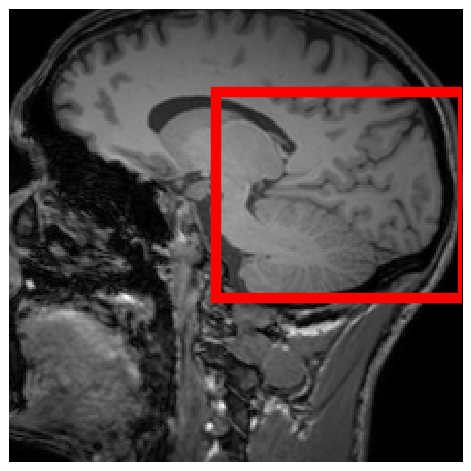
\includegraphics[width=2.5cm,height=2.5cm]{include/grp2/factor4/012-HH-1211-T1/012-HH-1211-T1_images__35} &
			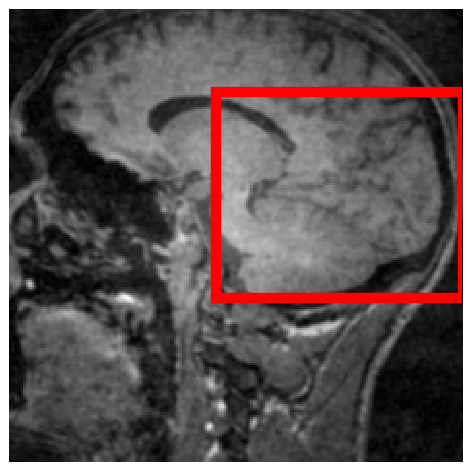
\includegraphics[width=2.5cm,height=2.5cm]{include/grp2/factor4/012-HH-1211-T1/012-HH-1211-T1_images__zeroPadding_35} & 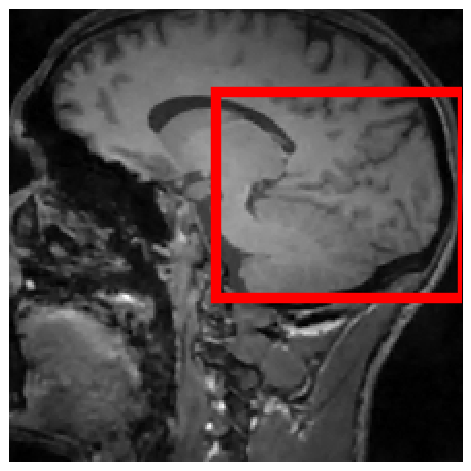
\includegraphics[width=2.5cm,height=2.5cm]{include/grp2/factor4/012-HH-1211-T1/012-HH-1211-T1_images__CS_35} & 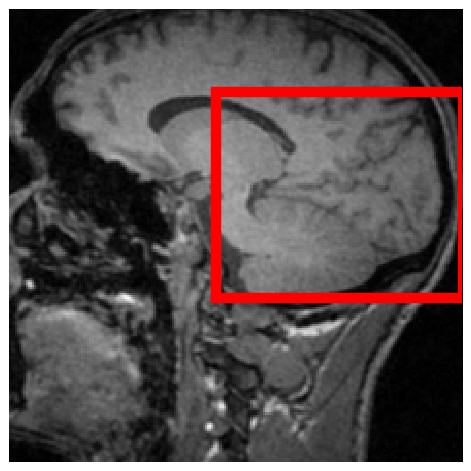
\includegraphics[width=2.5cm,height=2.5cm]{include/grp2/factor4/012-HH-1211-T1/012-HH-1211-T1_images__IMCNNL2TUNE_35} & 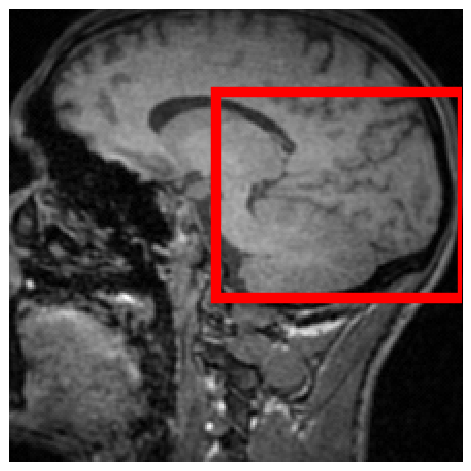
\includegraphics[width=2.5cm,height=2.5cm]{include/grp2/factor4/012-HH-1211-T1/012-HH-1211-T1_images__predict_35}
			
			\tabularnewline
			
			\multirow{1}{0.05cm}[1.3cm]{\begin{turn}{90} {\footnotesize Zoom in} \end{turn}} &
			
			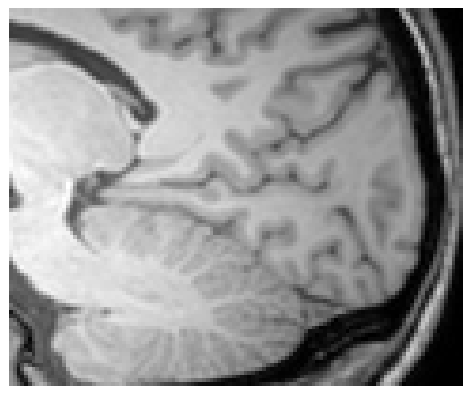
\includegraphics[width=2.5cm,height=2.5cm]{include/grp2/factor4/012-HH-1211-T1/012-HH-1211-T1_images__zoom_35} &
			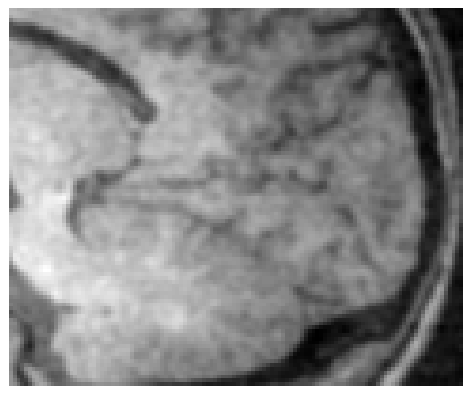
\includegraphics[width=2.5cm,height=2.5cm]{include/grp2/factor4/012-HH-1211-T1/012-HH-1211-T1_images__zeroPadding_zoom_35} & 
			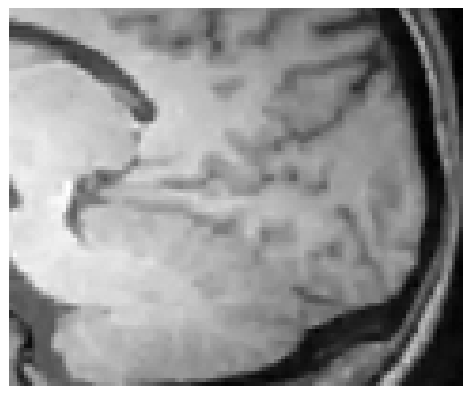
\includegraphics[width=2.5cm,height=2.5cm]{include/grp2/factor4/012-HH-1211-T1/012-HH-1211-T1_images__CS_zoom_35} & 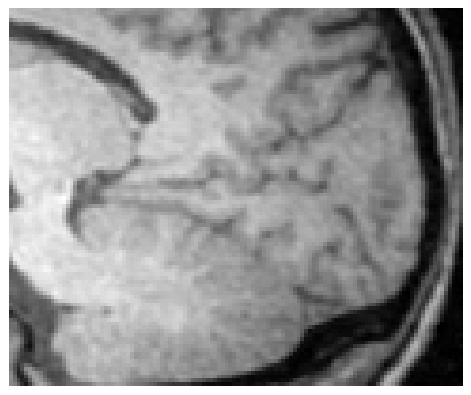
\includegraphics[width=2.5cm,height=2.5cm]{include/grp2/factor4/012-HH-1211-T1/012-HH-1211-T1_images__IMCNNL2TUNE_zoom_35} & 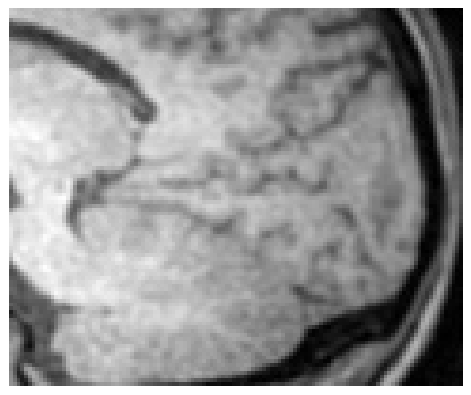
\includegraphics[width=2.5cm,height=2.5cm]{include/grp2/factor4/012-HH-1211-T1/012-HH-1211-T1_images__predict_zoom_35}
			
			\tabularnewline
			
			\multirow{2}{0.05cm}[1.4cm]{\begin{turn}{90} {\footnotesize Brain} \end{turn}} & 
			
			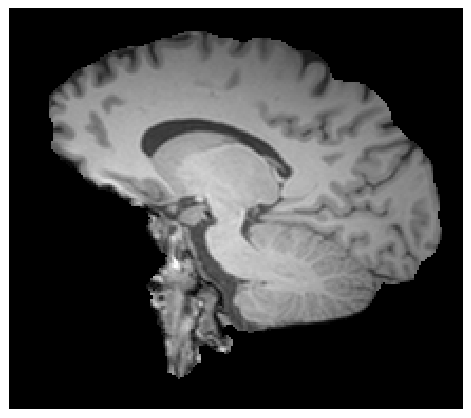
\includegraphics[width=2.5cm,height=2.5cm]{include/grp2/factor4/012-HH-1211-T1/012-HH-1211-T1_brains__35} &
			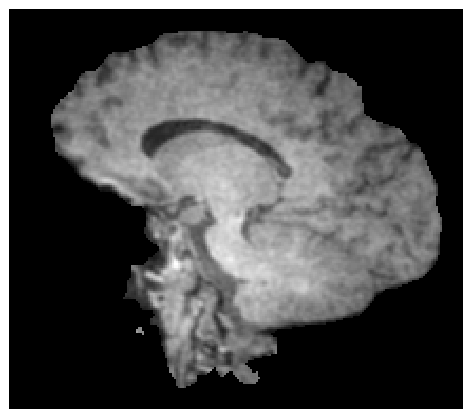
\includegraphics[width=2.5cm,height=2.5cm]{include/grp2/factor4/012-HH-1211-T1/012-HH-1211-T1_brains__zeroPadding_35} & 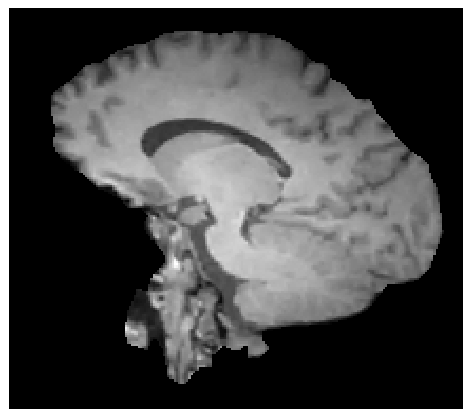
\includegraphics[width=2.5cm,height=2.5cm]{include/grp2/factor4/012-HH-1211-T1/012-HH-1211-T1_brains__CS_35} & 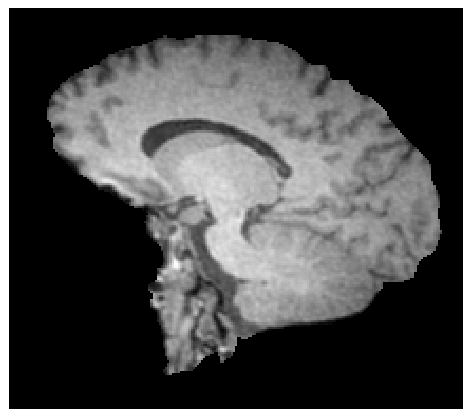
\includegraphics[width=2.5cm,height=2.5cm]{include/grp2/factor4/012-HH-1211-T1/012-HH-1211-T1_brains__IMCNNL2TUNE_35} & 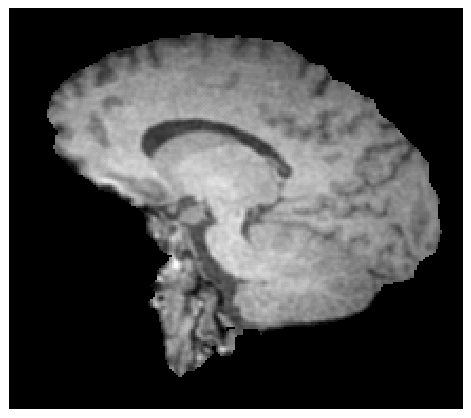
\includegraphics[width=2.5cm,height=2.5cm]{include/grp2/factor4/012-HH-1211-T1/012-HH-1211-T1_brains__predict_35}
			
			\tabularnewline
			
			\multirow{2}{0.05cm}[1.7cm]{\begin{turn}{90} {\footnotesize Segmentation} \end{turn}} &
			
			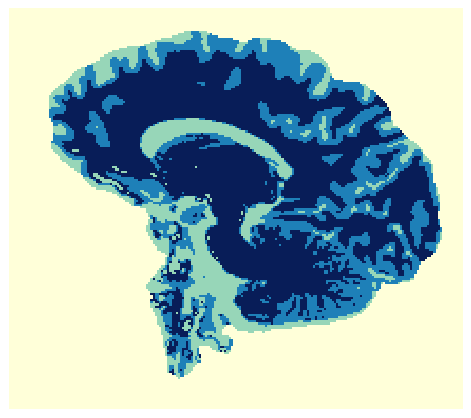
\includegraphics[width=2.5cm,height=2.5cm]{include/grp2/factor4/012-HH-1211-T1/012-HH-1211-T1_segs__35} &
			\includegraphics[width=2.5cm,height=2.5cm]{include/grp2/factor4/012-HH-1211-T1/012-HH-1211-T1_segs__zeroPadding_35} & \includegraphics[width=2.5cm,height=2.5cm]{include/grp2/factor4/012-HH-1211-T1/012-HH-1211-T1_segs__CS_35} & \includegraphics[width=2.5cm]{include/grp2/factor4/012-HH-1211-T1/012-HH-1211-T1_segs__IMCNNL2TUNE_35} & \includegraphics[width=2.5cm,height=2.5cm]{include/grp2/factor4/012-HH-1211-T1/012-HH-1211-T1_segs__predict_35}
			
			
		\end{tabular}
		\par\end{raggedleft}
	\raggedright{}\caption{\textcolor{black}{\footnotesize{}Examples of reconstructed MR images from under-sampled k-space - Factor 4.}}
	\label{fig:example_factor_4} 
\end{figure}

% Examples factor 2.5
\begin{figure}[H]
	%	\begin{raggedright}
	\begin{raggedleft}
		%		\begin{tabular}{>{\centering}b{0.2cm}lcccc}
		\hspace*{-2cm} \begin{tabular}{cccccc}
			& \multicolumn{1}{c}{\footnotesize Original} & {\footnotesize Zero-filled} & {\footnotesize CS-MRI} & {\footnotesize IM-CNN-L2} & {\footnotesize Proposed}\tabularnewline
			\multirow{1}{0.05cm}[1.8cm]{\begin{turn}{90} {\footnotesize Reconstructed} \end{turn}} &
			
			\includegraphics[width=2.5cm,height=2.5cm]{include/grp2/factor2/019-Guys-0702-T1/019-Guys-0702-T1_images__78} &
			\includegraphics[width=2.5cm,height=2.5cm]{include/grp2/factor2/019-Guys-0702-T1/019-Guys-0702-T1_images__zeroPadding_78} & \includegraphics[width=2.5cm,height=2.5cm]{include/grp2/factor2/019-Guys-0702-T1/019-Guys-0702-T1_images__CS_78} & \includegraphics[width=2.5cm,height=2.5cm]{include/grp2/factor2/019-Guys-0702-T1/019-Guys-0702-T1_images__IMCNNL2TUNE_78} & \includegraphics[width=2.5cm,height=2.5cm]{include/grp2/factor2/019-Guys-0702-T1/019-Guys-0702-T1_images__predict_78}
			
			\tabularnewline
			
			\multirow{1}{0.05cm}[1.3cm]{\begin{turn}{90} {\footnotesize Zoom in} \end{turn}} &
			
			\includegraphics[width=2.5cm,height=2.5cm]{include/grp2/factor2/019-Guys-0702-T1/019-Guys-0702-T1_images__zoom_78} &
			\includegraphics[width=2.5cm,height=2.5cm]{include/grp2/factor2/019-Guys-0702-T1/019-Guys-0702-T1_images__zeroPadding_zoom_78} & 
			\includegraphics[width=2.5cm,height=2.5cm]{include/grp2/factor2/019-Guys-0702-T1/019-Guys-0702-T1_images__CS_zoom_78} & \includegraphics[width=2.5cm,height=2.5cm]{include/grp2/factor2/019-Guys-0702-T1/019-Guys-0702-T1_images__IMCNNL2TUNE_zoom_78} & \includegraphics[width=2.5cm,height=2.5cm]{include/grp2/factor2/019-Guys-0702-T1/019-Guys-0702-T1_images__predict_zoom_78}
			
			\tabularnewline
			
			\multirow{2}{0.05cm}[1.4cm]{\begin{turn}{90} {\footnotesize Brain} \end{turn}} & 
			
			\includegraphics[width=2.5cm,height=2.5cm]{include/grp2/factor2/019-Guys-0702-T1/019-Guys-0702-T1_brains__78} &
			\includegraphics[width=2.5cm,height=2.5cm]{include/grp2/factor2/019-Guys-0702-T1/019-Guys-0702-T1_brains__zeroPadding_78} & \includegraphics[width=2.5cm,height=2.5cm]{include/grp2/factor2/019-Guys-0702-T1/019-Guys-0702-T1_brains__CS_78} & \includegraphics[width=2.5cm,height=2.5cm]{include/grp2/factor2/019-Guys-0702-T1/019-Guys-0702-T1_brains__IMCNNL2TUNE_78} & \includegraphics[width=2.5cm,height=2.5cm]{include/grp2/factor2/019-Guys-0702-T1/019-Guys-0702-T1_brains__predict_78}
			
			\tabularnewline
			
			\multirow{2}{0.05cm}[1.7cm]{\begin{turn}{90} {\footnotesize Segmentation} \end{turn}} &
			
			\includegraphics[width=2.5cm,height=2.5cm]{include/grp2/factor2/019-Guys-0702-T1/019-Guys-0702-T1_segs__78} &
			\includegraphics[width=2.5cm,height=2.5cm]{include/grp2/factor2/019-Guys-0702-T1/019-Guys-0702-T1_segs__zeroPadding_78} & \includegraphics[width=2.5cm,height=2.5cm]{include/grp2/factor2/019-Guys-0702-T1/019-Guys-0702-T1_segs__CS_78} & \includegraphics[width=2.5cm]{include/grp2/factor2/019-Guys-0702-T1/019-Guys-0702-T1_segs__IMCNNL2TUNE_78} & \includegraphics[width=2.5cm,height=2.5cm]{include/grp2/factor2/019-Guys-0702-T1/019-Guys-0702-T1_segs__predict_78}
			
			
		\end{tabular}
		\par\end{raggedleft}
	\raggedright{}\caption{\textcolor{black}{\footnotesize{}Examples of reconstructed MR images from under-sampled k-space - Factor 2.5.}}
	\label{fig:example_factor_2.5} 
\end{figure}



%-----------------------------BIBLIOGRAPHY--------------------%
%\vspace{-0.3cm}
\bibliography{paper}


\end{document}
